\chapter{Locality aware dynamic searchable encryption meets forward and backward privacy}\label{ch:iodse}
We focus on the problem of I/O-efficient Dynamic Searchable Encryption (DSE), i.e., schemes that perform well when executed with the dataset on-disk. Towards this direction, for HDDs, schemes have been proposed with good \emph{locality} (i.e., low number of performed non-continuous memory reads) and \emph{read efficiency} (the number of additional memory locations read per result item). \neww{Similarly,} for SSDs, schemes with good \emph{page efficiency} (reading as few pages as possible) have been proposed. However, the vast majority of these works are limited to the \emph{static} case (i.e. no dataset modifications) and the {only} dynamic scheme fails to achieve forward and backward privacy, the de-facto leakage standard in the literature. In fact, prior related works (Bost [CCS'16] and Minaud and Reichle [CRYPTO'22]) claim that I/O-efficiency and forward-privacy are two \emph{irreconcilable} notions.
% while they propose new I/O efficient Dynamic Searchable Encryption but without forward/backward privacy. 
Contrary to that, in this work, we ``reconcile'' {for the first time} forward and backward privacy with I/O-efficiency for DSE both for HDDs and SSDs. We propose two families of DSE constructions which also improve the state-of-the-art (non I/O-efficient) both asymptotically and experimentally. Indeed, some of our schemes improve the in-memory performance of prior works. \neww{ At a technical level, we revisit and enhance the \emph{lazy de-amortization} DSE construction by Demertzis et al. [NDSS'20], transforming it into an I/O-preserving one. Importantly, we introduce an oblivious-merge protocol that merges two equal-sized databases without revealing any information, effectively replacing the costly oblivious data structures with more lightweight computations.}


%At a technical level, we revisit and improve the \emph{lazy de-amortization} DSE \neww{construction} of Demertzis et al. [NDSS'20] into an I/O-preserving one. Importantly, we \new{introduce an oblivious-merge protocol which merges two equal-sized databases obliviously, and} replaces the costly oblivious data structures.
%with more lightweight and simpler-to-implement oblivious sorting.

%At a technical level, we revisit and refine the \emph{lazy de-amortization} DSE \neww{construction} of Demertzis et al. [NDSS'20] into an I/O-preserving one. Importantly, we \new{introduce a protocol which merges two equal-sized databases obliviously, and} replaces the costly oblivious data structures with more lightweight and simpler-to-implement oblivious sorting. %\todo{1. explain novelty}
%\tblue{add one line about oblivious merge.}
% DSE schemes for HDDs and SSDs, while at the same time 

% In this area, many recent works achieve the  of forward-and-backward privacy; however, none of these simultaneously achieves good I/O-performance when running from disk storage.
% % (forward privacy nullifies the leakage during updates; backward privacy controls during search the leaked information about deleted records).
\section{Preliminaries} \label{sec:prelim}
\noindent\textbf{Notation.} Let $(x';y')\leftrightarrow P(x;y)$ denote a protocol execution between a 
client and a server, {which may consist of multiple rounds of communication}, and $(x';y')\leftarrow A(x;y)$ 
denote an algorithm execution, with no communication between client and server---$x$ and $x'$ are the 
input and output for the client, and $y$ and $y'$ are the input and output for the server.  
We denote by $\lambda \in \mathds{N}$ a security parameter and by $v(\lambda)$ a negligible function in $\lambda$. \textsf{PPT} stands for \textsf{P}robabilistic \textsf{P}olynomial-\textsf{T}ime. $\D$ is a collection of $n$ documents with identifiers $id_1, \ldots, id_n$. A document contains a set of keywords from a dictionary $\Delta$. 
%$D(w)$ is the set of documents that contain keyword $w$.
 %to the set of identifiers of the documents that contain it. Let the database, denoted as $DB$, consists of keyword-identifier  %pairs of the form $\pair{w}{id}$. There are a total of $N$ entries in $DB$.
Let $DB$ consist of $N$ tuples of the form $(w,id,op)$--file $id$ contains keyword $w$, and $op$ is either $add$ or $del$, which denotes whether the tuple is for an insertion or deletion. $DB(w)$ is the set of identifiers of documents that contain keyword $w$. We use $n_w$ to denote $|DB(w)|$, i.e. the result size of keyword $w$. 
The aforementioned tuples can be expanded to $(w,id,op,rank,n_w)$, where $0 \leq rank < n_w$. $EDB$ denotes the encrypted database/index stored in the server. 
   
 %The acronym PPT stands for probabilistic polynomial-time.
 %Our searchable encryption protocols are executed 
 %between a client and a server in an interactive way. 
%  The notation $(x';y')\leftrightarrow P(x;y)$ denotes a protocol 
%  execution, where $x$ and $x'$ are the input and output for the client, and $y$ and $y'$ 
%  are the input and output for the server.

\smallskip\noindent\textbf{Pseudo Random Functions (PRFs) \cite{katz2020introduction}.} A PRF function  $F : {\{0, 1\}}^{\lambda} \times {\{0, 1\}}^{*} \rightarrow
{\{0, 1\}}^{*}$ is a two input function where the first input is the \textit{key} and the second is the input $x$. $F$ can be distinguished from a truly random function by a \textsf{PPT} adversary only with negligible probability $v(\lambda)$.  

% \medskip\noindent\textbf{Pseudorandom Functions.}
% Let $Gen(1^{\lambda}) \in \{0, 1\}^{\lambda}$ be a
% key generation function, 
% and $F : {\{0, 1\}}^{\lambda} \times {\{0, 1\}}^{\ell} \rightarrow
% {\{0, 1\}}^{\ell'}$ be a pseudorandom function (PRF) family. 
% $F$ is a secure PRF family if for all PPT adversaries Adv,
% $|Pr[K \leftarrow Gen(1^{\lambda}); 
% Adv^{F(K,\cdotp)}(1^{\lambda}) = 1]-Pr[Adv^{R(\cdotp)}(1^{\lambda}) = 1]| \leq v(\lambda)$, 
% where $R : {\{0, 1\}}^{\ell} \rightarrow {\{0, 1\}}^{\ell'}$ is a truly random function.


% \begin{figure}
% \begin{tabular}{|c|c|}
% \hline
% symbol & Definition \\
% \hline
% \hline
% $\lambda$ & security parameter \\
% \hline
% $v(\lambda)$ & negligible function in $\lambda$ \\
% \hline
% $w$ & keyword \\
% \hline
% $\Delta$ & dictionary of keywords \\
% \hline
% $n$ & total number of documents \\
% \hline
% $\D = \{d_1, \ldots d_n\}$ & set of documents \\
% \hline
% $\I = \{id_1, \ldots id_n\}$ & set of unique identifiers  \\
% & per document \\
% \hline

% $D:\Delta \rightarrow P(\I)$ & 
%                 $D(w)$ returns the document \\
%                 &  identifiers that contain $w$ \\
%                 \hline
% $\pair{w}{id}$ & keyword-identifier pair \\
% \hline
% $DB$& the database : collection of   \\
% & keyword-identifier pairs, i.e. \\
% & if $id \in D(w)$ then $\pair{w}{id} \in DB$ \\
% \hline
% N & total number of keyword-identifier \\
% & pairs i.e. $N = |DB| = \Sigma_{w\in\Delta}|D(w)|$ \\
% \hline
% $EDB$ & Encrypted $DB$ \\
% \hline
% \end{tabular}
% \end{figure}

\smallskip\noindent{\textbf{Dynamic Searchable Encryption (DSE).}} 
A DSE scheme  $\Sigma$ consists of a $\texttt{Setup}$ algorithm, and (possibly interactive) protocols $\texttt{Search}$ and $\texttt{Update}$--$\Sigma=(\texttt{Setup},\texttt{Search},\texttt{Update})$.
\begin{itemize}
    \item $(K,\sigma ;EDB) \leftarrow \texttt{Setup}(\lambda,N)$ takes as input the security parameter 
    $\lambda$ and $N$. Returns $EDB$ to the server, and the secret key $K$ and local state $\sigma$ to the client.
    
    \item $(res,K,\sigma;EDB) \leftrightarrow\texttt{Search}(K, w, \sigma; EDB)$ is a protocol for searching keyword $w$. The output of this protocol is the query result $res$ (i.e., $DB(w)$). The protocol may or may not modify $K$, $\sigma$ and $EDB$. 
    
    \item $(K,\sigma;EDB) \leftrightarrow\texttt{Update}(K, (w,id,op), \sigma ; EDB)$ is a protocol that inserts/removes $\pair{w}{id}$ to/from the DB--$op = add/del$. The protocol may modify $K$, $\sigma$ and $EDB$. {This protocol modifies $EDB$ and may modify $K$ and $\sigma$.}
\end{itemize}
{{The \texttt{Search} and \texttt{Update} algorithm/protocols for the schemes presented in section \ref{sec:de-amortized} also include an additional parameter $\Gamma$, which is an instance of a static SE scheme}\footnote{\new{$\Gamma$ is a static searchable encryption scheme such that $\Gamma = (\texttt{KeyGen},$ $\texttt{Setup},$ $\texttt{Search})$.}.}}

Following~\cite{bost2016ovarphiovarsigma,bost2017forward,ghareh2018new,SDa}, we start from an empty database. Given an input $DB$ of size $N$, the client populates $EDB$ by calling the $\texttt{Update}$ protocol $N$ times. Other works ~\cite{etemad2018efficient,kim2017forward} equivalently modeled updates in document granularity, i.e., inserting or 
deleting an entire document. We focus on retrieving only the document identifiers upon $\texttt{Search}$; the client may retrieve the documents separately if needed. This leads to a straightforward leakage formulation and is more natural for database queries (e.g.,~\cite{compress,Kamara16,Seal}).

% Following~\cite{bost2016ovarphiovarsigma,bost2017forward,ghareh2018new,SDa}, we assume that we start with an empty database by running $\texttt{Setup}$.Given a $DB$ of size $N$, 
% the client first instantiates the empty database by running $Setup$, 
% followed by $N$ calls to $Update$ to ``populate" the $EDB$. Other works ~\cite{etemad2018efficient,kim2017forward}
% have modeled different definitions of update, e.g. inserting or 
% deleting an entire document from the database. We argue that it is 
% functionally equivalent as it can be decomposed into multiple calls of 
% our version of $Update$. We have also omitted the fact 
% that after performing a $Search$, the client might
% make an additional step to retrieve the actual documents.}


\smallskip\noindent{\textbf{DSE--Leakages \& Forward/Backward privacy.}}
The standard security of a DSE scheme is parametrized by a leakage function $\lp = (\lp^{Stp}, \lp^{Srch}, \lp^{Updt})$. $\lp^{Stp}$ corresponds to the leakage during the setup phase--in our case it reveals size of the database $N$; %\tgreen{the rest have no example} 
$\lp^{Srch}$ corresponds to the leakage during search queries; $\lp^{Updt}$ corresponds to the leakage during update queries. %We discuss  $\lp^{Srch}$ and $\lp^{Updt}$ in more detail below. 
{\emph{Search pattern} leakage reveals which searches
are related to the same $w$, and \emph{access pattern} leakage reveals
$DB(w)$ during a search for $w$. \emph{Access pattern} leakage
is unavoidable if the client retrieves the actual files
with an additional round of communication with the server; schemes
that avoid this leakage (e.g. by storing files in oblivious data structures) 
are referred as \emph{result hiding} schemes.}

A secure DSE scheme with leakage $\lp$ should reveal nothing to an adaptive \textsf{PPT}\footnote{\new{An adaptive \textsf{PPT} decides its next step based on its previously observed leakages/search results.}} adversary about the database $DB$ other than the leakage $\lp$. This is formally captured by a standard real/ideal 
% experiment presented in Figure \ref{fig:games} in the Appendix \ref{append:secGames}---for more details see \cite{ShiNDSS14,ghareh2018new,bost2017forward}.
%@@
experiment presented in the extended version---for more details see \cite{ShiNDSS14,ghareh2018new,bost2017forward}.


%with two games RealSSE, IdealSSE following the definitTion of \cite{ShiNDSS14}.
% \medskip\noindent{\textbf{Leakages.}}
% One of the main design goals of an SE scheme is that the leakages associated with it should be as minimal as it can be. But in order to make the scheme useful for real world applications, some leakages are tolerated. 
% During the setup phase, the (maximum) number of entries of $DB$ 
% %and size of the documents 
% is revealed to the server. This leakage is unavoidable and is called the $total~leakage$. During searches and updates few other kinds of leakages occur. \emph{Search pattern} reveals if two queries are for the same keyword. \emph{Access pattern} reveals the documents in the result of a query. \emph{Total updates} reveals total number of times entries pertaining to a keyword $w$ is inserted and deleted (also referred as $n_w$). \emph{Response length} reveals the number of document identifiers in the query result of a keyword $w$, i.e. it reveals $|D(w)|$ (also referred to as $n_w$).
% ORAM based techniques are most commonly used to hide search and access pattern, while padding is used to hide $n_w$ and $n_w$.
% %\paragraph{\textbf{Leakage profile.}}
% Leakage profile of a particular SE scheme is represented as a collection of these above mentioned leakage patterns. 
% %An SE scheme $\Sigma$ is said to be correct if the returned result is correct for every query \cite{cash2014dynamic}. 
% The security of an SE scheme is parametrized by a leakage function $\lp = (\lp^{Stp}, \lp^{Srch}, \lp^{Updt})$ which captures the information revealed to the server or a passive attacker. $\lp^{Stp}$ corresponds to the leakage during setup phase, $\lp^{Srch}$ corresponds to the leakage during search  queries, and $\lp^{Updt}$ corresponds to the leakage during update queries. A secure SE scheme with leakage $\lp$ should reveal nothing about the database $DB$ other than the leakage, $\lp$, defined for it. \change{This is formally captured by a standard real/ideal experiment with two games RealSSE, IdealSSE following the definition of \cite{ShiNDSS14}.}
Forward and backward privacy~\cite{ShiNDSS14,bost2017forward} have become the de-facto security guarantees for modern DSE.

\noindent\underline{\textit{Forward privacy} (\textbf{FP}):} limits the information revealed due to updates. In particular, an $\lp$-adaptively secure DSE is forward private \textit{iff} the update leakage function $\lp^{Updt}$ can be written as: $\mathcal{L}^{Updt}({op},w,{id})=\mathcal{L'}^{Updt}({op},id)$ where $\mathcal{L'}$ is a stateless function, {$op=add/del$, and $id$ is a file identifier}. {Particularly, it should be impossible to tell whether an insertion is for a new keyword or a previously inserted/searched one}.\newline
\noindent\underline{\textit{Backward privacy} (\textbf{BP}):} ensures that during searches the server does not learn the identifiers of deleted documents that contained the searched keyword $w$. Bost et al.~\cite{bost2017forward} proposed various formulations for this property.
% three types of backward privacy (BP-I, BP-II, BP-III) with different leakage patterns, from Type-I which reveals the least information to Type-III which reveals the most. 
Here, we target backward private schemes that reveal the identifiers of (non-deleted) documents currently containing $w$ (known as $TimeDB(w)$ leakage) and the timestamps and type (i.e. insertion and deletion) of all prior updates for $w$ (known as $Updates(w)$ leakage). This corresponds to the \textbf{BP-II} definition from~\cite{bost2017forward} %(see Appendix \ref{append:BP} for more details). 
%@@
(see the extended version for more details).
{$TimeDB(w)$ accounts for the leakage from retrieving the actual files; but we focus only on retrieving the document identifiers during \texttt{Search}, and we never use it in our proofs as none of our constructions explicitly leaks $TimeDB(w)$.

\begin{definition}[\cite{bost2017forward}] \label{def:adpSec}
{A DSE scheme $\Sigma$ is $\lp$-adaptively-secure with forward and backward privacy, 
\textit{iff} $\mathcal{L}^{Updt}({op},w,{id}) = \mathcal{L}^{'}({op})$ 
and $\mathcal{L}^{Srch}(w)$  $=\mathcal{L}^{''}({TimeDB}(w),{Updates}(w))$ 
\textbf{and} \textit{iff} for any adaptive \textup{\textsf{PPT}} adversary $\adv$ 
~issuing polynomially many queries $q$, there exists a stateful \textup{\textsf{PPT}} simulator 
\textup{$\sim$}=$(SimSetup,~SimSearch,~SimUpdate)$ such that 

$|\Pr[{Real}^{\textsf{\emph{DSE}}}_{\adv}(\lambda,q)=1]-\Pr[{Ideal}^{\textsf{\emph{DSE}}}_{\adv,\sim,\mathcal{L}}(\lambda,q)=1]| < v(\lambda)$, where $\mathcal{L}^{'}$ 

and $\mathcal{L}^{''}$ are stateless functions; $op$ is insertion or deletion, and $id$ is a file identifier.}
% (BP-II_ functionand it is forward    scheme that supports single-keyword additions/deletions is forward private \textit{iff} the update leakage function  $\mathcal{L}^{Updt}$ can be written as:
% $\mathcal{L}^{Updt}({op},w,{id})=\mathcal{L'}^{Updt}({op},id)$
% where $\mathcal{L'}$ is a stateless function, {$op=add/del$, and $id$ is a file identifier}.
\end{definition}

% document $d$ containing keyword $w$ is deleted before a search for
% $w$, then the result of this search does not reveal anything about $d$. Backward privacy is categorized into three types. (a) Type-I/BP-I reveals only the identifiers of documents currently containing the searched keyword and timestamp of when the documents were inserted, (b) Type-II/BP-II additionally reveals the timestamps and type (i.e. insertion and deletion) of all prior updates for the searched keyword, (c) Type-III/BP-III also reveals for each deletion which insertion it canceled. 
% The following definitions will help us formally define backward privacy ~\cite{bost2017forward}.


%Dynamic symmetric searchable encryption (DSE) leaks additional information to what described above due to the update queries. 
% A dynamic SE is considered to be secure if it satisfies two additional security notions: forward and backward privacy.
% A scheme is forward private if an update does not reveal if the keyword
% pertaining to this update have been queried before. Achieving forward privacy for dynamic SE schemes is important as otherwise it suffers from adversarial document-injection attacks \cite{Seal}. 


% \begin{definition}[\cite{bost2017forward}]
% An $\mathcal{L}$-adaptively-secure DSE scheme that supports single-keyword additions/deletions is forward private \textit{iff} the update leakage function  $\mathcal{L}^{Updt}$ can be written as:
% $\mathcal{L}^{Updt}({op},w,{id})=\mathcal{L'}^{Updt}({op},id)$
% where $\mathcal{L'}$ is a stateless function, {$op=add/del$, and $id$ is a file identifier}.
% \end{definition}


% Backward privacy ensures that if a
% document $d$ containing keyword $w$ is deleted before a search for
% $w$, then the result of this search does not reveal anything about $d$. Backward privacy is categorized into three types. (a) Type-I/BP-I reveals only the identifiers of documents currently containing the searched keyword and timestamp of when the documents were inserted, (b) Type-II/BP-II additionally reveals the timestamps and type (i.e. insertion and deletion) of all prior updates for the searched keyword, (c) Type-III/BP-III also reveals for each deletion which insertion it canceled. 
% The following definitions will help us formally define backward privacy ~\cite{bost2017forward}.

% \change{Let $Q$ be a list that has one entry for each query executed. The entry for a search is of the form $(u,w)$ where $u$ is the query timestamp and $w$ is the searched keyword. Entry for an update is $(u,op,(w,id))$.
% %where $op=add/del$ and $id$ is the document identifier.
% For a keyword $w$, the function \textbf{TimeDB}($w$) returns 
% the list of all timestamp/identifier pairs of keyword $w$ that have been added to $DB$ and not subsequently deleted. }
% \begin{align*}
% \textbf{TimeDB}(w) = \{(u, {id}) \;| \;(&u, {add}, (w, {id})) \in Q \\ &\text{and }
% \forall u', (u', {del}, (w, {id})) \notin Q\}
% \end{align*}
% \textbf{Updates}($w$) function returns the timestamp of all insertion and deletion operations for $w$ in $Q$. 
% \begin{align*}
% \textbf{Updates}(w) =& \{u | (u, {add}, (w, {id})) \in Q \\
%  & \text{ or }~(u, {del}, (w, {id})) \in Q\}.
% \end{align*}
% Funtion \textbf{DelHist}($w$) returns all 
% (insertion timestamp, deletion timestamp) pairs revealing
% which deletion corresponds to which insertion for keyword $w$. 
% \begin{align*}
% \textbf{DelHist}(w) = \{(u^{add},u^{del})\; | \;&\exists\; {id} : (u^{add}, {add}, (w, {id})) \in Q\\ &\text{and }
% (u^{del}, {del}, (w, {id})) \in Q\}
% \end{align*}
% It is clear that the leakage of these three functions is progressively increasing. 
% We are now ready to formally define backward privacy with different types of leakage.

%The strongest backward privacy definition is the type I which reveals just currently existing documents having keyword $w$, their insertion time, and the total number of updates on each keyword. The formal definition of this statement is:

% \begin{definition}[\cite{bost2017forward}]\label{def-bp1}
% An $\mathcal{L}$-adaptively-secure SE scheme has backward privacy:

% 	\begin{itemize}
% 		\item []\textbf{Type-I} \textbf{(BP-I):} \textit{iff} $\mathcal{L}^{Updt}({op},w,{id}) = \mathcal{L}^{'}({op})$, and\\
% 		$\mathcal{L}^{Srch}(w) = \mathcal{L}^{''}(\textbf{TimeDB}(w),n_w)$.
% 		\item[] \textbf{Type-II}\textbf{ (BP-II):} \textit{iff} $\mathcal{L}^{Updt}({op},w,{id}) = \mathcal{L}^{'}({op},w)$, and
% 		$\mathcal{L}^{Srch}(w) = \mathcal{L}^{''}(\textbf{TimeDB}(w),\textbf{Updates}(w))$.
% 		\item[] \textbf{Type-III (BP-III):}		\textit{iff}\\ $\mathcal{L}^{Updt}({op},w,{id}) = \mathcal{L}^{'}({op},w)$, and\\	$\mathcal{L}^{Srch}(w) = \mathcal{L}^{''}(\textbf{TimeDB}(w),\textbf{DelHist}(w))$.	
% 	\end{itemize}

% where $\mathcal{L}^{'}$ and $\mathcal{L}^{''}$ are stateless {functions}.
% \end{definition}
% \change{
% Note that the above definition assumes schemes leak the documents that
% currently contain $w$ in order to account for the leakage from actually retrieving the files. Namely, \textbf{TimeDB}($w$) function explicitly reveals the indexes of  returned documents.} 
% %While none of our schemes reveals this information directly, we still account for it as
% %part of our leakage.

\smallskip\noindent{\textbf{DSE for HDDs: Locality/Read-Efficiency/Update Locality/Update Cost/Space}.}
To scale SE to big data using external memory (i.e., HDD drives),  SE schemes with ``small'' locality and read efficiency have been proposed before. \emph{Locality} is defined as the number of \emph{non-contiguous} memory accesses made during the search by the server. \emph{Read-efficiency} is the ratio of the total amount of data read/retrieved during the search over the actual query result size (for querying a keyword $w$)---see \cite{cash2014locality} for formal definitions. 
%Cash and Tessaro \cite{cash2014locality} proved that in any secure SE scheme with both optimal locality $\bO(1)$ and optimal read efficiency $\bO(1)$ requires $\omega(N)$ space. The intuition behind this lower bound is that in a scheme with optimal locality, read efficiency and linear space, an attacker/server can observe the locations of some queries, as well as the non-accessed ones and infer statistical information about the entire input dataset, i.e., learn information about queries which we have not requested. 
Cash and Tessaro \cite{cash2014locality} proved that any secure SE scheme with both optimal locality $\bO(1)$ and optimal read efficiency $\bO(1)$ requires $\omega(N)$ space. %The intuition behind this lower bound is that schemes with optimal locality, read efficiency, and linear space allow attackers/servers to infer statistical information about the entire input dataset (even for non-requested queries) using information about some accessed queries and observing the non-accessed memory locations. 
%\todo{6.Give the definition of I/O efficiency metrices }
For locality-aware DSE schemes, in addition to the "search" and "static" efficiency, i.e., (i) locality, (ii) read-efficiency and (iii) space, we focus on two update metrics: (iv) update-locality, i.e., the number of \emph{non-contiguous} memory accesses during an update and (v) update asymptotic cost, i.e., the {asymptotic} cost of one update (i.e., insert/delete one $(w,id,op)$ tuple). 
%See Appendix \ref{append:metrics} for the exact definitions.
%@@
See the extended version for the exact definitions.

%\tgreen{the text here sounds like locality and update cost are novel definition}
%\tpurp{--I dont think so.}

% \begin{itemize}
%     \item \emph{Update Locality:} is defined as the number of \emph{non-contiguous} memory accesses during an update.
%     \item \emph{Update Overhead:} is defined as the cost/overhead of one  update (i.e., insert/delete one $(w,id,op)$ tuple).\footnote{Other works consider batch updates (or operate in document granularity). For that case, we can define  \emph{Update Efficiency} as the ratio of the total amount of data read/retrieved during a batch of updates over the batch size.}
% \end{itemize}


% \emph{Update Locality:} The number of total \emph{non contiguous} memory accesses during an update  \\ 
% \emph{Update Overhead:} The ratio of total amount of data read (retrieved) during an update
%                             to the actual amount of data that corresponds to the update 

% The amount of space required to store EDB is called its $space~overhead$. The ideal goal is to construct an SE scheme with optimal space overhead ($\bO(N)$), optimal locality ($\bO(1)$), and optimal read efficiency ($\bO(1)$). But Cash and Tessaro \cite{ct14} proved that achieving optimality in all these three metrices is impossible. Specifically, they prove a lower bound: ``any scheme must be sub-optimal in either its space overhead, its locality, or its read efficiency". 

% \paragraph{\textbf{Dynamic Locality-aware SSE.}}
% Unlike static SE schemes, for Dynamic Locality-aware schemes no such lower bound 
% has been proven yet. Moreover, as DSE schemes support updates, we formally define 
% two new metrices : \\
% \emph{Update Locality:} The number of total \emph{non contiguous} memory accesses during an update  \\ 
% \emph{Update Overhead:} The ratio of total amount of data read (retrieved) during an update
%                             to the actual amount of data that corresponds to the update 

\smallskip\noindent{\textbf{DSE for SSDs: Page-Efficiency/Space}.}
Bossuat et al. \cite{BFF21} proposed a new I/O-efficiency dimension for SSDs, which is called \emph{page efficiency}---SSD performance mainly depends on page efficiency, aiming at reading as few memory pages as possible. More formally, \emph{page efficiency} is the ratio of the total number of pages that the server accesses (using SE) over the optimal number of accessed pages in a plaintext case. %\todo{6. Give the definition of I/O efficiency metrices } 
For page-efficient DSE schemes, in addition to the "search" and "static" efficiency dimensions, i.e., (i) page-efficiency and (ii) space, we focus on (iii) update efficiency, i.e., the number of pages accessed 
 during one update (i.e., insert/delete one $(w,id,op)$ tuple) and (iv) update asymptotic cost (i.e., {asymptotic cost} of insert/delete of one $(w,id,op)$ tuple).
%See Appendix \ref{append:metrics} for the exact definitions.
%@@
See the extended version for the exact definitions.



%@@ more detailed explanation Page Efficient literature
% \tblue{
% \noindent{\textbf{DSE for SSDs--Page-Efficiency/Space}.}
% Locality and read efficiency are not meaningful metrics when solid state drives (SSD) are used as the underlying 
% storage device. For SSDs, the memory accesses are done in terms of memory pages, and the performance 
% is mainly determined by the number of these pages accessed, regardless of whether they are contiguous 
% pages or not. Bossuat et al. \cite{BFF21} present a new criterion called \emph{page efficiency} 
% to capture performance of an SE scheme whose data is stored on SSDs.
% The \emph{page efficiency} is defined as the number of pages that 
% the server must access to process a client's query, 
% divided by the number of pages of the plaintext answer to
% the query. In the same paper the authors presented a \emph{page efficient} static 
% searchable encryption scheme (\textbf{PE-SE}) called Tethys. 
% Storage efficiency in this model is the number of
% pages needed to store the encrypted database, divided by the number of 
% pages of the plaintext database. Tethys offers $\bO(1)$ page efficiency 
% and $\bO(1)$ storage efficiency, but the client storage is not optimal $ \bO{p \log \lambda}$,
% where $p$ is the page size and $\lambda$ is the security parameter. 
% The authors in \cite{BFF21} claims that page efficiency is 
% an excellent predictor of SSD performance and they supported their claim with experiments as well.
% In~\cite{LocalLayeredSSECrypto22} Minaud and Reichle presented two DSE schemes.
% The first one is a dynamic page efficient SE (\textbf{PE-DSE})
% scheme, called \LayeredSSE, that offers 
% \tpurp{$\bO(\log \log N )$} page efficiency, and $\bO(1)$ storage efficiency and client 
% storage. The second scheme takes a PE-SE scheme as 
% an input parameter and runs it along with an overflowing SE (which they call OSSE) scheme. 
% %The basic idea is that if a keyword list overflows, then the 
% %overflowing items will be stored in 
% %the PE-SE scheme, rest will be stored in the OSSE scheme.
% They use a variant of One-Choice Allocation as their OSSE scheme, 
% that supports new updates but ignores the overflowing items.
% There are $\log N$ instances of the PE-SE scheme. If a keyword-list
% of size $k$ overflows then the overflowing items
% go to $\ceil{\log{k}}^{th}$ instance of PE-SE.
% This scheme offers $\bO(1)$ locality, 
% $\bO(1)$ storage efficiency, and \tpurp{$\bO(\log \log N )$}
% read efficiency, but under the condition that the longest list
% is of size $N^{1-\frac{1}{\log \log N}}$. These schemes do not
% ensure $FP$ and $BP$.
% }
% \tblue{
% For PE-DSE schemes, we classify the \emph{page efficiency} metric into two:
% \emph{Search Page Efficiency} and \emph{Update Page Efficiency}.
% \begin{itemize}
%  %\itemsep-0.3em 
%  \item \emph{Search Page Efficiency:} the number of pages that 
% the server must access to process a search query, 
% divided by the number of pages of the plaintext answer to the search query
%  \item \emph{Update Page Efficiency:}  the number of memory pages accessed 
%  during one update (i.e., insert/delete of one $(w,id,op)$ tuple).%\footnote{Similar to \emph{Update Efficiency}, one can define  \emph{Update Page Efficiency} as the ratio of the total number of pages read/retrieved during a batch of updates over the size of the batch in terms of pages.}
% \end{itemize}
% }

\smallskip\noindent{\textbf{Oblivious sort.}}
An oblivious sorting algorithm sorts an array of $N$ elements without leaking information about the relative ordering of the input elements \cite{aks,zigzag,bitonic,ngai2024distributed}. We use the oblivious bucket sort~\cite{bucketSort}, 
which has $\bO(N \log N$) time complexity, and uses a temporary client 
storage { of two buckets, where one bucket contains} 512 elements. 
%and merge sort as the \emph{non-oblivious} sort that bucket sort requires for the last step. 
We can decompose bucket sort into $N \log N/\gamma$ rounds of $\bO(\gamma)$ work per round (e.g., for $\gamma = O(\log N)$ the oblivious bucket sort can be completed in $N$ rounds). We highlight that fetching $\bO(\gamma)$ elements from disk requires always $\bO(1)$ locality, since accesses are performed on a {bucket granularity}, \new{and on consecutive buckets}---
%see Figure \ref{fig:bucketSort} and \ref{fig:mergeSort} in the Appendix \ref{append:bucketLoc} for more details.
%@@
see the extended version for more details.

%@@ More detailed discussion for o-sort 
%



\smallskip\noindent{\textbf{Oblivious compaction.}}
Given an array of $N$ elements, some of which are tagged with bit 1, and the rest 
with bit 0, an oblivious compaction \cite{compact1,compact2,godrichOblComp} 
generates an output in which all the 
elements tagged with bit 1 appear before all the elements tagged with bit 0, without leaking the information of which elements were tagged with bit 1 or 0.  
Our constructions need the compaction to be
order preserving, i.e. the relative ordering of the elements tagged with bit 1/0 do not change after the compaction. We use the oblivious bucket sort~\cite{bucketSort} mentioned above for performing order preserving compaction.


\smallskip\noindent\textbf{Oblivious Maps}($\textsc{OMAP}$)\cite{wang2014oblivious,dauterman2021snoopy}.
%\label{append:omap}
An oblivious map is a data structure that supports oblivious read/get and write/put functionality for encrypted $(key,value)$ pairs (i.e., oblivious hash map). That is, all same-length operation sequences appear indistinguishable. $\textsc{OMAP}$ has the following algorithms/protocols: (i) $\textsc{OMAP}$.$\texttt{Setup}$ initializes an empty data structure with maximum capacity $N$ blocks, (ii) $\textsc{OMAP}$.$\texttt{put}$ adds/overwrites a $(key,value)$ pair, and (iii) $\textsc{OMAP}$.$\texttt{get}$ returns the $value$ of a given $key$. We have used the AVL tree based implementation by Wang et al.~\cite{wang2014oblivious} on top of PathORAM~\cite{stefanov2013path}. For a map with capacity $N$, each oblivious access requires $\bO(\log^2 N)$ operations/accessed-blocks, $\bO(\log N)$ roundtrips, and $\bO(\log^2 N)$ locality---see~\cite{wang2014oblivious} for more details. 

% Goodrich’s oblivious compaction algorithm \cite{godrichOblComp} runs in time $\bO(N \log N)$ 
% and is order-preserving.
% This algorithm accesses array locations in a fixed order using a $\log N$ deep routing network that
% shifts each element a fixed number of steps in every layer. 
%\tpurp{check the paper to see how to de-amortize it, or we can 
%replace it with bucket oblivious sort, which has the same time complexity}


% \paragraph{\textbf{Oblivious sort.}}
% An oblivious sorting algorithm is a sorting algorithm that always compares the elements in the input dataset in the same order regardless of their values. Bitonic sort (also known as Batcher's sort)~\cite{bitonicsort}, is an oblivious sorting algorithm which sorts $N$ elements in $\bO(N\log^2 N)$ time.
% %and with $\bO(\log^2 N)$ locality. 
% The algorithm assumes $N$ to be in power of 2 (padded if not). It \textbf{\textit{compares-and-swaps}} elements in $\log N$ phases. The $i$th phase has $i$ subphases, with $\frac{N}{2}$ \textit{compare-and-swap}s in each subphase. Hence a total of - $$\frac{N}{2}\cdot{\sum_{i=1}^{\log N}i}=\frac{N}{2}\cdot \frac{\log N (\log N +1))}{2}= \frac{N \log N (\log N +1)}{4}$$ \textit{compare-and-swap}s are required to produce a sorted output. Because, the \textit{compare-and-swap}s happen in a fixed schedule, the algorithm can be decomposed into fixed number of rounds, with fixed number of \textit{compare-and-swap}s in each round. For instance, if we decide to execute $\gamma$ number of \textit{compare-and-swap}s per round (ideally $\gamma$ divides $\frac{N \log N (\log N +1)}{4}$ ) then the algorithm will need $\ceil{\frac{N \log N (\log N +1)}{4\gamma}}$ rounds to complete. In one of our schemes the client downloads the necessary $2\gamma$ elements, to perform the $\gamma$ \textit{compare-and-swap}s, then it encrypts those elements with fresh encryptions and sends them back to the server.


% Asharov et al.~\cite{bucketSort} presents an oblivious bucket
% sort that sorts the elements in three steps: 
% \emph{Oblivious Random Bin Assignment (ORB)}, \emph{Oblivious Random Permutation (ORP)}
% and \emph{Non-oblivious Sorting}. During \emph{ORB} the elements are 
% assigned a random key and are randomly distributed into $B$ buckets with $Z/2$
% elements in each bucket ($B= 2N/Z$). $Z/2$ dummy elements are added in each of the bucket. Then, $\log B +1$ rounds of merge-splits are performed, 
% with $B/2$ merge-splits in each round. The main idea is that, 
% during the $i^{th}$ round of merge-splits, every two buckets 
% at distance $2^i$ are fetched by the client and their elements are
% assigned to correct output buckets based on the $i^{th}$ bit 
% of their random key. The two output buckets are written back to level $i+1$.
% During the \emph{ORP} step, 
% each bin is fetched separately by the client, 
% their dummy elements are removed and the real elements are permuted. The \emph{ORP} can be combined together with the last round of $OBA$ . Once all the bins are permuted, any \emph{non-oblivious} sort can be performed to sort the elements. They have proved that composition of these three steps results into an \emph{Oblivious sort}.
% As a total of $B/2 (\log B +1)$ merge-splits are performed, the runtime 
% of this algorithm is $\bO(N\log N)$, if the \emph{non-oblivious} sort
% also has $\bO(N \log N)$ runtime. In our construction
% we have used merge sort as the \emph{non-oblivious} sort. 
% Since elements of a bucket are 
% always stored in contiguous memory locations,
% locality of fetching a bucket is always $\bO(1)$. 

%\todo{7.Clarify which scheme targets which storage and which metrices}
%\todo{20. Explain 1C/2C/NlogN in depth. Explain what superbin is.} 

%\smallskip
\smallskip\noindent{\textbf{One-Choice Allocation.}}
Asharov et al.~\cite{onechoice} presented 
the One-Choice Allocation scheme 
(we will refer to it as \OneChoice) that offers optimal locality,
optimal space overhead and $\bO(\log N \log \log N)$ read efficiency.
Given a database of size $N$, this scheme allocates an 
array of $m={N}/{\log N \log\log N}$ bins, each of 
size $3\log N \log \log N$\footnote{\new{The bins overflow with negligible probability when the bin size is set to $3\log N \log \log N$ for \OneChoice}.}. For each keyword $w$ it computes a hash value $h(w)$, and stores the $i^{th}$ document identifier
in the bin $(h(w) + i)mod~m$. Bins are filled up with $dummy$ entries, if not full.
% The formal description of 1C is provided 
% in Figure \ref{alg:1C}, and Figure \ref{fig:allSEschemes} shows an example in the Appendix. 
%@@
The formal description of 1C is provided the extended version. 
%in Figure \ref{alg:1C}, and Figure \ref{fig:allSEschemes} shows an example in the Appendix. 


\smallskip\noindent{\textbf{Two-Choice Allocation.}}
Asharov et al. also presented the Two-Choice Allocation 
(\TwoChoice) in \cite{onechoice}.
For a database of size $N$, this scheme offers optimal locality and space overhead and 
$\bO((\log\log N)^A(\log$$\log$$\log N)^2)$ read efficiency 
assuming keyword list sizes $<N^{1-1/(\log\log N)^A}$, 
for a constant $A \geq 1$. This scheme allocates an 
array of $m={N}/{(\log\log N)^A (\log \log \log N)^2}$ bins, each bin with  
size $z{\cdot}(\log\log N)^A$ ($\log$$\log$$\log N)^2$, where $2\leq z \leq 4$ (we use $A=1$).
The keyword lists are padded to be nearest power of 2 and stored in decreasing length order. 
For list for $w$, first
it divides bins into groups of $sb = \frac{m}{n_w}$ \emph{superbins}; \neww{i.e. each \emph{superbin} consists of $n_w$ bins.} Then two superbins are chosen with two hash functions: 
$h_1(w)\% sb$ and $h_2(w)\%sb$. \neww{Finally,} the superbin that has \neww{minimal load} stores the list for $w$. 
%Formal description \neww{and an example} of 2C are in Figures \ref{alg:2C} \neww{and \ref{fig:allSEschemes}} in Appendix. 
%@@
The formal description of 2C is provided the extended version. 

\smallskip\noindent{\textsf{\textbf{NlogN}} \textbf{Scheme.}}
The third scheme presented by Asharov et al. in~\cite{onechoice} 
offers optimal locality and read efficiency at the cost of
$\bO(\log N)$ storage overhead, i.e. a total of $\bO(N\log N)$ storage. We highlight this scheme provides optimal page efficiency. This scheme consists of $(\log N +1)$ hash tables, each of size $N$. The keyword-lists are padded so that their length becomes 
nearest power of 2. The $k^{th}$ hash-table stores lists of size $2^k$.  
%The pseudocode of the \NlogN\ scheme is provided in Figure \ref{alg:NlogN}, and Figure \ref{fig:allSEschemes} shows an example in the Appendix. 
%@@
The pseudocode and more details of the \NlogN\ scheme are provided in the extended version. %Figure \ref{alg:NlogN}, and Figure \ref{fig:allSEschemes} shows an example in the Appendix. 
Demertzis et al. \cite{Demertzis17} proposed a variation of the \NlogN\ scheme in which only $s$ of the above mentioned hash tables are stored; $s$ is evenly distributed (i.e. the server stores the levels $\{0, x, 2x, \ldots (s-1){\cdot}x \}$, 
where $x$ is set to be $\lceil{\frac{\log N+1}{s}}\rceil$). In the worst case, 
a keyword-list is divided into smaller $\bO(N^{\frac{1}{s}})$ chunks. 
This scheme achieves optimal read efficiency, $\bO(N^{\frac{1}{s}})$ locality and 
has a $\bO(s)$ space overhead, and $\bO(\text{min}\{N^{\frac{1}{s}}/p, p\})$ page efficiency ($p$ denotes the memory page size). We refer to this scheme as \sN.






%  levels starting from 
% level 0, instead of storing $\ell = (\log N+1)$ levels
% (where $s$ can be as small as 2). Specifically, a value of $p$ is set to be $\ceil{\frac{\ell}{s}}$, 
% and the server stores the levels $\mathcal{L} = \{0, p, 2p, \ldots (s-1){\cdot}p \}$.
% The keyword-list of a keyword $w$ is divided into smaller chunks 
% of size $2^j$ and stored in the level $j$ if $2^j \leq |DB(w)| < 2^i$ for $i,j\in \mathcal{L}$.
% This idea is first introduced in \cite{Demertzis17}
% by We will refer to this scheme as \textsf{Ns}.
% This scheme achieves optimal read efficiency, $\bO(N^{\frac{1}{s}})$ 
% locality and has a $\bO(s)$ space overhead.}



%\tpurp{Description of \Tethys\ is in the appendix.}




%\paragraph{\textbf{LayeredSSE}.}
\smallskip\smallskip\noindent{\textbf{Encrypted dictionary.}}
\new{In our DSE constructions (in section \ref{sec:dseio}) along with the 
encrypted index we have an encrypted dictionary. The 
encrypted dictionary maintains a keyword to keyword-counter 
mapping, i.e. keyword $w$ maps to $|DB(w)|$. To perform searches 
in \OneChoice, \TwoChoice, \NlogN, and \Ns\ schemes the keyword-counter
is required (to know how many bins to fetch, or which levels to search). 
%Because our DSE constructions in section 
%\ref{sec:dseio} use these above mentioned static SE schemes, we needed to 
%maintain this encrypted dictionary as well. 
We will refer to the encrypted 
dictionary as $EDB.\Dict$ and the encrypted index as $EDB.\Index$. % in the rest of the paper.
For an index with $N$ entries the size of $EDB.\Dict$ is at most $N$,
as there can be at most $N$ distinct keywords.}

%\tblue{We should decribe the $EDB.\Dict$ briefly here, it will 
%help us describe the locality/read-efficiency in section \ref{sec:SDalocality}}

%\paragraph{Result hiding SE.} \tblue{Add a short description of it. }
% In a response-hiding scheme, the adversary can not infer
%whether two different responses have overlapping records, thus
%making reconstruction harder. \tred{I think we should not use the term "result-hiding" (result-pattern hiding) at all}
\section{DSE---I/O efficiency meets Forward/Backward Privacy}\label{sec:dseio}
%This section presents our I/O efficient DSE schemes which are the first that achieve both good I/O performance and forward/backward privacy. In Section \ref{sec:SDalocality}, we use
% the \SDa\ transformation proposed by Demertzis et al.\cite{SDa} which transforms static SE schemes to dynamic ones with forward/backward privacy. 
% Our observation is that if we use I/O efficient static SE schemes in the \SDa\ transformation, then the I/O efficiency will be preserved in the produced dynamic ones while maintaining forward/backward privacy. In Sections \ref{sec:de-amortized}, we focus on the more challenging task of providing de-amortized I/O efficient constructions with forward/backward privacy; we provide a new \emph{oblivious merge} framework which achieves the above goals, and we provide three instantiations of this framework---the dynamic de-amortizated \OneChoice, \TwoChoice, and \NlogN\ schemes. 
\neww{
This section introduces our I/O efficient DSE schemes, which are the first to simultaneously achieve good I/O performance and forward/backward privacy. In Section \ref{sec:SDalocality}, we apply the \SDa\ transformation, as proposed by Demertzis et al.\cite{SDa}, in conjunction with I/O efficient static SE schemes. In Section \ref{sec:de-amortized}, we address the more challenging task of offering de-amortized I/O efficient constructions that ensure forward/backward privacy. Here, we introduce a novel \emph{oblivious merge} framework to meet these objectives and present three implementations of this framework: the dynamic de-amortized \OneChoice, \TwoChoice, and \NlogN\ schemes.}


%Later in section \ref{sec:eval} we show our experimental evaluation for these schemes along with the \sN\ scheme for some specific values of s.
%\tgreen{What about \sN scheme?}





\subsection{Amortized Constructions using \SDa \textup{\cite{SDa}}\label{sec:SDalocality}}

\noindent{\textbf{Overview of \SDa[$\cdot$].}} 
% \todo{2. general overview of the transformation} 
% Recently, Demertzis et al~\cite{SDa} proposed a generic compiler called \SDa~that yields a forward/backward private DSE scheme from any result hiding static SE scheme. 
% The high-level idea of \SDa~is that the result of  $N$ updates is stored as a 
% collection of $\log N $ indexes (0$th$ through $(\log N-1)th$),
% where the $i$th index (denoted as $EDB_i$) is of size $2^{i}$. For each new update
% the client runs the \texttt{Setup} of the underlying static SE
% scheme to create an index of size 1 (i.e. $EDB_0$).
% Whenever two indexes of the same size (say $z$) exist, 
% they are downloaded by the client, and the setup of the
% static scheme is called to ``merge'' them into a
% single new index of size $2z$, amortizing the cost of updates.
% Searches are 
% performed in each index independently.  
% In Figure \ref{fig:SDaex1}, we provide an example of an update in \SDa. 
Demertzis et al.~\cite{SDa} introduced a compiler, \SDa, that converts any result hiding static SE scheme into a forward/backward private DSE scheme. The essence of \SDa\ is to store the results of $N$ updates across $\log N$ indexes (ranging from 0$th$ to $(\log N-1)th$). The $i$th index ($EDB_i$) has a size of $2^{i}$. With each update, the client initializes the static SE scheme (using SE's \texttt{Setup}) to produce and upload an encrypted index with size 1 ($EDB_0$). When two same-sized indexes emerge (in server), the client downloads, decrypts and combines them into a doubled size index, amortizing the cost of updates. Searches are performed in each index independently. Figure \ref{fig:SDaex1} shows an update example using \SDa. 
%The optimized pseudocode for \SDa, as depicted in Figure \ref{fig:SDaex1}, can be found in Figure \ref{fig:Scheme1} in the Appendix.
%@@
The optimized pseudocode for \SDa, as depicted in Figure \ref{fig:SDaex1}, can be found in the extended version.

%Figure \ref{fig:SDaex1} shows and update example for \SDa.}We provide the pseudocode of \SDa\ \cite{SDa}(with the optimization shown in Figure \ref{fig:SDaex1}) in Figure \ref{fig:Scheme1} in the Appendix.
%An update example in \SDa is depicted in Figure \ref{fig:SDaex1}.






%\tgreen{Let us assume that the indexes $EDB_0$ and $EDB_1$ already exist, while a new element needs to be inserted. The new insertion causes the creation of $EDB_0$ (Step 1). At this point two 
%$EDB_0$ indexes exist, hence they are downloaded and merged 
%to create $EDB_1$. When $EDB_1$ is uploaded to the server (Step 2), again
%two $EDB_1$ indexes exist, so the two $EDB_1$
%are downloaded and merged to create $EDB_2$ (Step 3). -- repetitive} The above steps are shown 
%with gray arrows in Figure \ref{fig:SDaex1}, while 
% The \neww{black} arrow indicates an equivalent optimized version of \SDa\ in which the client looks for the smallest index level $k$, that does not exist at the server and downloads all the indexes \new{(along with the keyword dictionaries)} $EDB_0,\ldots, EDB_{k-1}$, then creates $EDB_{k}$ with the entries of $EDB_0,\ldots, EDB_{k-1}$ along
% with the new entry. We provide the pseudocode of the original optimized version of \SDa\ from \cite{SDa}
% in Figure \ref{fig:Scheme1} in the Appendix.

In~\cite{SDa}, the authors 
 use \PiBas\cite{cash2014dynamic} as the underlying static SE scheme. 
\PiBas\ maps every $(w,id,op)$ tuple to a pseudo-random location 
(using a counter $cnt_w$ that is maintained locally for each keyword).
During search for $w$, all locations for {counter values} $1,\dots,cnt_w$
are accessed to retrieve the results. The results are decrypted and the deleted entries are filtered locally at the client. While this gives us a very simple and lightweight scheme, when it comes to I/O overhead, due to the pseudorandom 
placement,  the number of disk head movements (HDD case) and the number of fetched pages (SDD case) is equal to the result size. In other words, \SDa[$\cdot$] when applied to \PiBas\ gives a DSE with the worst possible \emph{search locality} and \emph{page efficiency}.


\begin{figure}[t!]
\centering
\scalebox{0.6}{
\begin{tikzpicture}
[%green = gray red=white blue=black yellow = light gray
greenball/.style={circle, draw=gray, fill=gray, thick, minimum size=7mm},
redball/.style={circle, draw=black, fill=white, thick, minimum size=7mm},
blueball/.style={circle, draw=black, fill=black, thick, minimum size=7mm},
yellowball/.style={circle, draw=gray, fill=gray!30, thick, minimum size=7mm},
grayball/.style={circle, draw=black, fill=gray, thick, minimum size=7mm},
bin/.style={cylinder, draw=black!70, fill=white, thick, minimum height=2.4cm, minimum width = 1cm, rotate=90},
bin2/.style={cylinder, draw=black!70, fill=white, thick, minimum height=1.3cm, minimum width = 1cm, rotate=90},
textbox/.style={rectangle, draw=white, fill=white, thick, minimum height=0.2cm},
box1/.style={rectangle, draw=black, fill=white, very thick, minimum height=2.8cm, minimum width=1.4cm},
box2/.style={rectangle, draw=black, fill=white, very thick, minimum height=2.8cm, minimum width=2.7cm},
box3/.style={rectangle, draw=black, fill=white, very thick, minimum height=1.6cm, minimum width=1.4cm},
myarrow1/.style={single arrow, draw=gray, fill=gray, 
      minimum width = 1mm, single arrow head extend=1mm,
      minimum height=1cm},
myarrow2/.style={single arrow, draw=black, fill=black, 
      minimum width = 1mm, single arrow head extend=1mm,
      minimum height=1.3cm},
myarrow3/.style={single arrow, draw=blue, fill=blue, 
minimum width = 0.09cm, single arrow head extend=0.05cm,
minimum height=0.7cm},
]
\node at (0.2,7.1) [blueball] (blueball)               {};
%\node at (0.5, 6.5) [myarrow3,rotate=-45] (a1) {};
%\draw[->] (0.5,6.7) -- (1,6) ;
\node at (0.3,6.4) [textbox] (tb) {insert};
\node at (0.5,5) [box3,label={south:$EDB_0$}] (firstbox) {} ;
 %\node at (0.5,5) [bin2] (bin2) {};
\node at (0.5,5) [greenball]      (ball3)     {};
\node at (2.18,5.6) [box1,label={south:$EDB_1$}] (b3) {};
  % \node at (2.2,5.5) [bin] (bin2) {};
 \node at (2.2,5.1) [yellowball]      (ball4)       {};
 \node at (2.2,6.1) [redball]      (ball5)   {};
  %\draw[->] (blueball.east) -- (firstbox.north);
  \node at (3.5, 5.5) [myarrow1,label={south:Step 1}] (a1) {};
   \node at (1.5, 3) [myarrow2,rotate=270,label={south:Optimized}] (a2) {};
\node at (5.08,6.6) [box3,label={south:$EDB_0$}] (b4) {} ;
 %\node at (5.1,6.5) [bin2] (bin1) {};
\node at (5.1,6.6) [blueball]      (ball3)   {};
\node at (5.08,4.3) [box3,label={south:$EDB_0$}] (b4) {} ;
 %\node at (5.1,4.2) [bin2] (bin1) {};
\node at (5.1,4.3) [greenball]      (d3)   {};
\node at (6.78,5.6) [box1,label={south:$EDB_1$}] (b3) {} ;
%   \node at (6.8,5.5) [bin] (bin2) {};
 \node at (6.8,5.1) [yellowball]      (ball4)        {};
 \node at (6.8,6.1) [redball]      (ball5)   {};
  \node at (5.9, 2.7) [myarrow1,label={north:Step 2},rotate=-90] (a2) {};
 \node at (1.15,0.6) [box2,label={south:$EDB_2$}] (b2) {} ;
% \node at (0.5,0.5) [bin] (bin2) {};
\node at (0.5,0.1) [blueball]      (ball3)  {};
\node at (0.5,1.1) [redball]      (d3)   {};
%\node at (1.8,0.5) [bin] (bin2) {};
 \node at (1.8,0.1) [greenball]      (ball4)    {};
 \node at (1.8,1.1) [yellowball]      (ball5)   {};

 \node at (3.5, 0.6) [myarrow1,label={north:Step 3},font=\small,rotate=180] (a1) {};
 \node at (4.98,0.6) [box1,label={south:$EDB_1$}] (b4) {} ;
 %\node at (5,0.5) [bin] (bin1) {};
\node at (5,0.1) [blueball]   (ball3)    {};
\node at (5,1.1) [greenball]      (d3)   
  {};
 \node at (6.78,0.6) [box1,label={south:$EDB_1$}] (b3) {} ;
  % \node at (6.8,0.5) [bin] (bin2) {};
 \node at (6.8,0.1) [yellowball]      (ball4)      {};
 \node at (6.8,1.1) [redball]      (ball5)    {};
\end{tikzpicture}
}
%\captionsetup{font=small}
\caption{Update in \SDa. Before the insertion of the new (black) entry three previous consecutive insertions have created EDB0 and EDB1. After the fourth insertion, two EDB0 indexes exist (Step 1), which are downloaded and merged to a single EDB1 of size 2 (Step 2). Now, two EDB1 indexes exist, which are downloaded and merged to a single EDB2 of size 4 (Step 3). The black arrow shows an optimized version of \SDa~where the intermediate steps are skipped.}
\label{fig:SDaex1}
\end{figure}


\smallskip\noindent{\textbf{I/O-efficient \SDa[$\cdot$].}} \neww{Our main observation here is that  when applied to an \emph{I/O-efficient} %result-hiding 
static scheme, the \SDa~transformation gives dynamic schemes with "good" I/O performance. %At a high level, the locality (for HDDs) or the page-efficiency (for SSDs) of the resulting DSE would have an additional factor of $\bO(\log N)$ as each index is queried independently. 
In fact, in the extended version we prove two theorems that state that the resulting \SDa[$\Gamma$] transformation 
will retain same \emph{space-overhead} as that for $\Gamma$, where as for \emph{locality}, \emph{read-efficiency} (for HDDs) and  \emph{page-efficiency} (for SSDs) an additional factor of $\bO(\log N)$ is introduced as each index is queried independently}

%queried independently.

%be the same as the underlying static SE plus a factor of $\bO(\log N)$ as each index is %queried independently. \todo{theorems}}

% can also lead to 
% In this work, we are concerned with \emph{locality} 
% of the DSE schemes. To improve \emph{locality}, 
% we can instantiate \SDa with any \emph{locality aware},
% result-hiding, static SE scheme. 
%\todo{7.Clarify which scheme targets which storage and which metrices}


\smallskip\noindent\textbf{Locality-aware \SDa[$\cdot$] (for HDDs).}
\neww{There exist various candidates for static locality-aware schemes, the \OneChoice\ and \TwoChoice\ schemes from \cite{onechoice} achieve optimal \emph{locality}, storage, and polylogarithmic \emph{read-efficiency}. The \NlogN\ scheme from \cite{onechoice} provides optimal \emph{locality} and \emph{read-efficiency} but increases storage. Other recent schemes are also introduced in \cite{TwoChoicePPCrypto18, Demertzis17, locCrypto18}.}
%There exist various candidates for static locality-aware schemes, namely the \OneChoice\ and \TwoChoice\ schemes of~\cite{onechoice} that have optimal \emph{locality} and storage, and polylogarithmic \emph{read-efficiency}, the \NlogN\ scheme~\cite{onechoice} with optimal \emph{locality} and \emph{read-efficiency} but blow-up the storage, as well as the more recent schemes of~\cite{TwoChoicePPCrypto18, Demertzis17,locCrypto18}. 


\smallskip\noindent\textbf{Page-Efficient \SDa[$\cdot$] (for SSDs).}
{\Tethys\ \cite{BFF21} and \NlogN\ \cite{onechoice} are candidates for static page-efficient schemes.}
%In \SDa[\Tethys] the results of a search can be distributed in at most $\log N$ levels. Let us assume a list of length $l (= l_0+l_1+\ldots + l_{\log N})$ is distributed into all the index levels. If the start and end points of the list are not aligned with server pages then total page accesses = $\Sigma_{i=0}^{\log N} (\frac{l_i}{p}+2) = \frac{l}{p}+2{\cdot}\log N$.  
% The amortized update overhead of \SDa[\Tethys] is $\bO(N \log N)$ 
% %\tblue{again calculation can be included in the appendix}, 
% since its setup is $\bO(N^2)$. 
% Similarly, the page efficiency of \SDa[\NlogN] is $\bO(\log N)$, and its amortized update overhead $\bO(\log^2 N)$ (since its page-efficiency is $\bO(1)$ and setup time is $\bO(N \log N)$ respectively). 
\neww{
Table~\ref{table:SDaLoc} shows various \SDa~instances from \emph{locality-aware} and \emph{page-efficient} static schemes. In this work, we emphasize the most practical I/O-efficient static SE schemes: \OneChoice\ and \TwoChoice\ (suitable for HDDs) and \NlogN 
 (compatible with both HDDs and SSDs). The security and forward/backward privacy of the DSE schemes resulting from the \SDa$[\cdot]$ transformation are directly derived from \cite[Theorem 1]{SDa}. {In the extended version we provide a more detailed 
discussion for \SDa[$\cdot$].}}

% Below, we focus on the instantiation of \SDa~with \OneChoice, denoted as \SDa[\OneChoice], 
% %\tblue{as it will be important for our de-amortized construction in Section~\ref{sec:de-amortized} -- we should remove this part}. \tpurp{Let us choose \OneChoice\ scheme and }
% to explain the locality and read-efficiency as stated in the Theorem \ref{thm:SDaLoc} above.
%  %,and on \SDa~with \Tethys, denoted \SDa[\Tethys].
% The $i^{th}$ index of \SDa$[\OneChoice]$ stores the
% real $2^i$ elements across $\ceil{{2^i}/{\log 2^i \log \log 2^i}}$ bins.
% %, where each bin can store upto $3{\cdot}\log 2^i \log \log 2^i$ elements\footnote{except indexes $EDB_0$ and $EDB_1$, which have 
% %a single bin each, with capacity 1 and 2 respectively}.
%  During a search, each index is searched by calling 
% \OneChoice.\Search, with locality $\bO(1)$, 
% as \emph{locality} of \OneChoice\ is $\bO(1)$.
% Since there are at most $\log N$ non-empty indexes: \new{$EDB_0.\Ind$, $EDB_1.\Ind$ \ldots $EDB_{\log N -1}.\Ind$, 
% and the corresponding $\log N$ dictionaries: $EDB_0.\Dict$, $EDB_1.\Dict$ \ldots $EDB_{\log N-1}.\Dict$, the total number of required I/Os is $2\log N$, i.e.} search locality for \SDa$[\OneChoice]$ is $\bO(\log N)$. 
% %(i.e. an I/O is needed for querying the dictionaries even if the corresponding index does not contain any result for the queried keyword).
% Read-efficiency for \SDa$[\OneChoice]$ is $\bO(\log N \log\log N + \log N)$; \new{the extra $\log N$ factor is added as $\log N$ keyword counter information is fetched from the $\log N$ dictionaries}. 
% The transformation preserves the storage overhead of \OneChoice, which is optimal. %($\bO(N)$). 
% Finally, regarding updates, the amortized update overhead is $\bO(\log N)$ as the setup time of \OneChoice~ is linear, and the update locality is $\bO(\log N)$ as at most $\log N$ indexes are fetched. Table~\ref{table:SDaLoc} provides different instantiations of the \SDa[$\cdot$] transformation with \emph{locality-aware} static SE schemes. We highlight that the amortized update overhead for \TwoChoice\ and \NlogN\ is $\bO(\log^2 N)$ since their setup time is $\bO(N \log N)$. 

%From Table~\ref{table:SDaLoc} one can see that \SDa$[\OneChoice]$ has higher {read-efficiency} than \SDa$[\PiBas]$. However, as our experimental evaluation shows (see Figure \ref{fig:}), the lower locality of the former makes it much more efficient when data is stored on hard-disk.

% \textit{Encrypted dictionary.} 
% \tpurp{we can remove it, as its already present in the original paper
% , and extra details provided in  the appendix \ref{append:locAware}}


% \tblue{During search, the client computes the first bin 
% for a keyword $w$ using the 
% \OneChoice~hash function $h(w)$. But, the client also 
% needs to know how many bins to fetch starting from the first bin.
% Hence, our modified \OneChoice~algorithm maintains an encrypted dictionary,
% that maps each unique keyword to its corresponding keyword-counter. 
% Please refer to Figure \ref{fig:1C} for the pseudocode of \OneChoice.
% Along with the encrypted bins (represented as $EDB.$\Ind, the server now
% stores the encrypted dictionary (represented as $EDB$.\Dict) as well. 
% }
% \tblue{
% \textit{Encrypted dictionary.} In section \ref{sec:prelim} we mentioned that 
% along with the database, the server also stores 
% an encrypted dictionary, that maps keywords to 
% the corresponding keyword-counters. As every 
% index level in \SDa~maintains a separate instance of \OneChoice\ ($EDB_0.\OneChoice$, $EDB_1.$$\OneChoice$, $\ldots$, $EDB_{\ell}.\OneChoice$ \tpurp{can we please change the notation here?}),
% every \SDa~index level now has an encrypted dictionary
%  ($EDB_0.\Dict$, $EDB_1.\Dict$, $\ldots$, $EDB_{\ell}.\Dict$).
% }
% %\tblue{
% %The dictionary is created using a \MAP~function (see Figure \ref{alg:encMap}). 
% %For a keyword $w$ and its keyword-counter $n_w$, 
% %\MAP~takes a $prf$ key, an $encryption$ key, $w$ and $n_w$ as inputs and returns a 
% %$(key, value)$ pair. The dictionary stores $value$ at position $key$.
% %The $value$ is the encryption of $n_w$, and the $key$ is 
% %produced from $w$ with the help of a pseudo-random function. 
% %}

% \smallskip\noindent\textbf{Page-Efficient \SDa[$\cdot$].}
% \todo{7.Clarify which scheme targets which storage and which metrices}
% \SDa\ can be instantiated with a static \emph{page-efficient} scheme, e.g., \Tethys\ \cite{BFF21} and \NlogN\ \cite{onechoice}. \Tethys\ fetches two pages from the server during search, hence it offers $\bO(1)$ \emph{search page efficiency}. So the page efficiency of \SDa[\Tethys] will be  $\bO(\log N)$ (since it will require two page accesses per index). 
% %In \SDa[\Tethys] the results of a search can be distributed in at most $\log N$ levels. Let us assume a list of length $l (= l_0+l_1+\ldots + l_{\log N})$ is distributed into all the index levels. If the start and end points of the list are not aligned with server pages then total page accesses = $\Sigma_{i=0}^{\log N} (\frac{l_i}{p}+2) = \frac{l}{p}+2{\cdot}\log N$.  
% The amortized update overhead of \SDa[\Tethys] is $\bO(N \log N)$ 
% %\tblue{again calculation can be included in the appendix}, 
% since its setup is $\bO(N^2)$. 
% Similarly, the page efficiency of \SDa[\NlogN] is $\bO(\log N)$, and its amortized update overhead $\bO(\log^2 N)$ (since its page-efficiency is $\bO(1)$ and setup time is $\bO(N \log N)$ respectively). 

%In worst case all the index levels are downloaded and merged to build the new index during update. In best case only  the smallest level is built. If we look closely we will see for a total of $i$ indexes, the $i$th index is built once, the $(i-1)$th index is built once, the $(i-2)$th  index is built twice, the $(i-3)$th index is built 4 times and so on. Taking the summation, we get for $N$ updates pages fetched $\approx \bO(N \log N /p)$, which results into the amortized \emph{update page efficiency} for one update to be $\bO(\log N /p)$.

%\begin{theorem}
%\tblue{Another theorem for PE-SE ?}
% \todo{14.Overall intuition of the proofs (for non-experts) }
% \smallskip\noindent\textbf{Security.} \new{The security and forward/backward privacy of 
% the DSE schemes resulting from \SDa$[\cdot]$ transformation follow directly from~\cite[Theorem 1]{SDa}.}
% \begin{theorem}\label{thm:scheme1}
% 	Assuming {\sf SE} is an adaptively-secure result-hiding static searchable encryption scheme, \SDd\ is an adaptively-secure DSE according to \textup{Definition~\ref{def:adpSec}} with $\mathcal{L}^{Updt}(\text{op},w,\text{id}) = \bot$  and  
% 	$\mathcal{L}^{Srch}(w) = \textbf{Updates}(w)$.
% %	(\text{TimeDB}(w),\text{Updates}(w))$.
% \end{theorem}
% \noindent\textit{Proof sketch.}
% Building a simulator {\sf Sim} is straight-forward, given the existence of a simulator ${\sf Sim}_{{\sf SE}} = \{SimInit_{{\sf SE}}, SimSearch_{{\sf SE}}\}$. $SimInit$ returns empty vector $EDB$ and initializes and update counter $upd=0$. During each update, $SimUpdate$ computes $j$ as the least significant zero bit position of $ upd$, runs a new instance ${\sf Sim}^{(j)}_{{\sf SE}}= \{SimInit^{(j)}_{{\sf SE}}, SimSearch^{(j)}_{{\sf SE}}\}$, executes $SimInit^{(j)}_{{\sf SE}}$ on input $2^j$, and sends the result to the adversary. It also terminates currently running instances of $SimInit^{(i)}_{{\sf SE}}$ for $i=0,\dots,j-1$, and increments $upd$. During a search for $w$, let $upd$ be the current update counter. $SimSearch$ receives as input $\textbf{Updates}(w)$.
% %and sets $n_w = |\textbf{Updates}(w)|$. 
% It then initializes values $t_0,\dots,t_{\lfloor\log upd\rfloor}$ to 0. For each entry $u \in \textbf{Updates}(w)$, it computes $i$ as the index in which the update with timestamp $u$ was stored (determined by $upd,u$) and increments $t_i$ by one. Finally for $j=0,\dots, \lfloor\log upd\rfloor$, it runs $SimSearch^{(j)}_{{\sf SE}}$ on input $t_j$, and sends all the outputs to the adversary.
% Assuming {\sf SE} is secure and result-hiding, and each instance ${\sf Sim}_{{\sf SE}}$ is spawned independently with fresh randomness, and given that the timestamp of an update fully determines the corresponding index structure for its entry, the transcript produced by {\sf Sim} is indistinguishable from the messages observed by the adversary during the real protocol execution. $\square$


\section{De-amortized constructions:LSDd}\label{sec:de-amortized}
Although \SDa provides a clean way to transform a static SE scheme to a dynamic one, its drawback is that it has amortized update cost. In the worst case an update may require rebuilding an index of size $N$ at once. 
Figure {app-fig:update} illustrates the above weakness of schemes with amortized update cost. 
In this section, we construct I/O efficient DSE schemes with de-amortized updates and with forward and backward privacy. 
Our starting point is the de-amortization strategy that Demertzis et al.~\cite{SDa} proposed for \SDa, called  \SDd\ (which is tailored on \PiBas \cite{cash2014dynamic}; {pseudocode of \PiBas\ can be found in the extended version}.
In this work, we introduce \LSDd, which is simpler than \SDd\ and separates the static-to-dynamic transformation from the underlying static SE scheme. 
We highlight that \LSDd\ is not a compiler; it is specifically tailored for certain schemes, namely \OneChoice, \TwoChoice, and \NlogN\ schemes. 
We present \LSDd\ primarily as a framework for the sake of clarity and concise presentation. 
Below, we explain the new \LSDd: \label{subsec:deamortized}

\begin{algorithm}
  %\caption{Voting Protocol}
  \caption{$(K,\sigma;EDB) \gets \setup(\lambda, N)$}
  \label{alg:setup}
  \begin{algorithmic}[1]
  \State $\ell \gets  \lceil{\log N}\rceil$;\quad 
$upd_{cnt} \leftarrow 0$;
\State Set matrix $P$ of size $(\ell+1){\cdot} 4$
\State $k_{rnd} \gets \RND.\keyGen(1^\lambda)$
\State $\sigma \leftarrow \{upd_{cnt}\}$ and $K \gets (k_{rnd},P)$
\State Initialize an empty $EDB$
\State \Return $EDB$ to Server and $(K,\sigma)$ to the Client
  \end{algorithmic}
\end{algorithm}

\begin{algorithm}
\caption{$(K,\sigma;EDB) \gets \setup(\lambda, N)$}
\begin{algorithmic}[1]
\State $\ell \gets  \lceil{\log N}\rceil$;\quad 
$upd_{cnt} \leftarrow 0$;
\State Set matrix $P$ of size $(\ell+1){\cdot} 4$
\State $k_{rnd} \gets \RND.\keyGen(1^\lambda)$
\State $\sigma \leftarrow \{upd_{cnt}\}$ and $K \gets (k_{rnd},P)$
\State Initialize an empty $EDB$
\State \Return $EDB$ to Server and $(K,\sigma)$ to the Client
%\State \Return $(K,\sigma)$ to the Client
\end{algorithmic}
\end{algorithm}


\begin{figure}
\begin{mdframed}	
  %\begin{multicols}{2}
 \underline{$(K,\sigma;EDB) \gets \setup(\lambda, N)$}
\begin{algorithmic}[1]
\State $\ell \gets  \lceil{\log N}\rceil$;\quad 
$upd_{cnt} \leftarrow 0$;
\State Set matrix $P$ of size $(\ell+1){\cdot} 4$
\State $k_{rnd} \gets \RND.\keyGen(1^\lambda)$
\State $\sigma \leftarrow \{upd_{cnt}\}$ and $K \gets (k_{rnd},P)$
\State Initialize an empty $EDB$
\State \Return $EDB$ to Server and $(K,\sigma)$ to the Client
%\State \Return $(K,\sigma)$ to the Client
\end{algorithmic}

\underline{$DB(w) \leftrightarrow {\Search}(K,\Gamma, q,\sigma ; EDB)$}
			%\underline{$\textsf{Search}(st_{\mathcal{C}},w, L)$}
			\begin{algorithmic}[1]
				%\State Parse the array of maps $EDB$ as set of indexes $L$; $\sigma$ as set of states $st$; K as a vector of secret keys ${\sf vec\_key}$ and compute $\ell = \lfloor \log N \rfloor$.
				%\State Parse state $st_{\mathcal{C}}$ as $(\lambda,{\sf vec\_key}, N)$. Compute $\ell = \lfloor \log N \rfloor$.
				\item[Client $\leftrightarrow$ Server:]
				\State $\mathcal{X}\leftarrow\emptyset$
				\For{$i=\ell \cdots 0$}
				\If {${\OLDEST}_i.\Ind \neq \emptyset$} 
    %\tpurp{the definition of $\Sigma.\Search$ does not have $2^i$ as a parameter, but we need it here, \Search also takes the static scheme $\Sigma'$ as an input parameter, should we change the definition ??}
				\State \hskip-0.7em$\mathcal{X} \leftarrow \mathcal{X} \; \cup$ {$\Gamma$.\Search}($K[i][0], q,\sigma;{\OLDEST}_i$)
				\EndIf
				\If {${\OLDER}_i.\Ind \neq \emptyset$}
				\State \hskip-0.7em$\mathcal{X}$ $\leftarrow$ $\mathcal{X}$ $\cup$ {$\Gamma$.\Search}($K[i][1],q,\sigma; {\OLDER}_i$)
				\EndIf
				\If {${\OLD}_i.\Ind \neq \emptyset$}
				\State \hskip-0.7em$\mathcal{X}$ $\leftarrow$ $\mathcal{X}$ $\cup$ {$\Gamma$.\Search}($K[i][2], q,\sigma;{\OLD}_i$)
				\EndIf
				\EndFor
				\item[Client:]
				%\State Decrypt entries of $\mathcal{X}$ with $K$ parse them as $(id,op)$
				\State $DB(w)\leftarrow\{id\; | \; (w,id,add)\in \mathcal{X} \land (w,id,del) \not\in \mathcal{X}\}$
				%\State \textbf{return} $(\mathcal{X},st_{\mathcal{C}}',\mathcal{I}')$.
			\end{algorithmic}
%\end{multicols}
\end{mdframed}
%\caption{\SDd,\LSDd: from {$\Gamma$=(\keyGen, \Setup, \Search)} to DSE (de-amortized version).}
\label{fig:SSEtoDSE1}
\end{figure}

\newcommand{\var}[1]{\text{\texttt{#1}}}
\newcommand{\func}[1]{\text{\textsl{#1}}}
\newcounter{phase}[algorithm]
\newlength{\phaserulewidth}
\newcommand{\setphaserulewidth}{\setlength{\phaserulewidth}}
\newcommand{\phase}[1]{%
  \vspace{-1.25ex}
  % Top phase rule
  \Statex\leavevmode\llap{\rule{\dimexpr\labelwidth+\labelsep}{\phaserulewidth}}\rule{\linewidth}{\phaserulewidth}
  \Statex\strut\textit{$\triangleright$ #1 }% Phase text
  % Bottom phase rule
  \vspace{-1.25ex}\Statex\leavevmode\llap{\rule{\dimexpr\labelwidth+\labelsep}{\phaserulewidth}}\rule{\linewidth}{\phaserulewidth}}
\setphaserulewidth{.7pt}

\begin{algorithm}
  \caption{Voting Protocol}
  \label{alg:phoenix-voting}
  \begin{algorithmic}[1]
    \phase{\textbf{as a replica k}} \\
    When replica \texttt{j} is suspected\\
    \hskip 1em broadcast $\langle VOTE, j, getLatestDec(\texttt{DecLog})$, \O $\rangle_{\sigma_{k}}$\\
  \vspace{0.1cm}
    When replica \texttt{j} is detected with Proof \\
    \hskip 1em broadcast $\langle VOTE, j, getLatestDec(\texttt{DecLog}), Proof \rangle_{\sigma_{k}}$\\
  \vspace{0.1cm}
    When received m : $\langle VOTE, j, Cert, Proof \rangle_{\sigma_{i}}$ from
    replica \texttt{i}\\
    \hskip 1em \textbf{if} \texttt{i} in \texttt{Conf} $\land$ \texttt{m.j} in
    \texttt{Conf} $\land$ isValidCert(\texttt{m.Cert})\\
\end{algorithmic}
\end{algorithm}

\begin{figure}%[!h]
%\begin{mdframed}	
\underline {$(K, \sigma; EDB) \leftrightarrow$ {\texttt{Update}$(K,(w,id,op),\Gamma,\sigma;EDB)$}}
%\underline {\sf Update$(op,w,id,st_{\mathcal{C}})$}
\begin{algorithmic}[1]
\item[Client $\leftrightarrow$ Server:]
\State Parse $K$ as $(k_{rnd},P)$ \Comment{$k_{rnd}$ is encryption key, $P$ is an array of PRF keys}
\For{$i=\ell, \dots, 1$}
\If {${\OLDEST}_{i-1}.\Ind \neq \emptyset \land {\sf OLDER}_{i-1}.\Ind \neq \emptyset$} \Comment{$\Gamma$ is \{\PiBas,\OneChoice,\TwoChoice,\NlogN\}}
\State{Execute the next $\gamma$ steps of $\Gamma$.\omerge$(K,\sigma,\OLDEST_{i-1},\OLDER_{i-1})$ and update $\NEW_i$} \label{alg:ssetodse1} 
\If {${\sf NEW}_i.\Ind$ is full}\label{sddalg:newfull}\Comment{Client can deduce this from $upd_{cnt}$}
\State Server sets ${\OLDEST}_{i-1}\leftarrow {\OLD}_{i-1}$  and ${\OLDER}_{i-1} \leftarrow \emptyset$ \label{sddalg:oldmove}
\If {${\OLDEST}_{i}.\Ind = \emptyset$} server sets ${\OLDEST}_{i} \leftarrow {\NEW}_{i}$ and client sets $P[i][0] \leftarrow P[i][3]$ \label{sddalg:newmove1}
\ElsIf {${\OLDER}_{i}.\Ind = \emptyset$} server sets ${\OLDER}_{i} \leftarrow {\NEW}_{i}$ and client sets $P[i][1] \leftarrow P[i][3]$ \label{sddalg:newmove2}
\Else {} server sets ${\OLD}_{i} \leftarrow {\NEW}_{i}$ and client sets $P[i][2] \leftarrow P[i][3]$ \label{sddalg:newmove3}
\EndIf
\State Client sets $P[i][3] \leftarrow$ {$\Gamma$}.{\texttt{KeyGen}}$(1^\lambda)$ \label{sddalg:keygen}
\EndIf
\EndIf
\EndFor
\State Client sets $P[0][3] \leftarrow$ {$\Gamma$}.{\texttt{KeyGen}}$(1^\lambda)$ \label{sddalg:keygen0}
			\State Client runs {$\Gamma$}.\setup($P[0][3]$, $(w,id,op)$) and sends the output to server who stores it as ${\sf NEW}_0$ \label{sddalg:new0full}
			\If {${\sf OLDEST}_0.\Ind = \emptyset$} server sets ${\sf OLDEST}_0 \leftarrow {\sf NEW}_0$ and client sets  $P[0][0] \leftarrow P[0][3]$ \label{sddalg:new0move2}
			\ElsIf {${\sf OLDER}_0.\Ind = \emptyset$} server sets ${\sf OLDER}_0 \leftarrow {\sf NEW}_0$ and client sets  $P[0][1] \leftarrow P[0][3]$ \label{sddalg:new0move3}
			\Else {} Server sets ${\sf OLD}_0 \leftarrow {\sf NEW}_0$ and client sets  $P[0][2] \leftarrow P[0][3]$ \label{sddalg:new0move3}
			\EndIf
			\State Client sets $upd_{cnt} \leftarrow upd_{cnt}+1$
\State \Return $EDB$ to Server and $(K,\sigma)$ to Client
			%\State Update $K, \sigma, EDB$ accordingly.
			%\State \textbf{return} $(K,\sigma,EDB)$.
		\end{algorithmic}
	%\end{mdframed}
	\caption{\SDd/\LSDd: from {$\Gamma$=(\keyGen, \Setup, \Search)} to DSE (de-amortized version).}
	\label{fig:SSEtoDSE2}
 %\vspace{-1.2em}
\end{figure}







\smallskip\noindent\textbf{Overview of \textbf{\LSDd[$\cdot$].}}  The main idea of \LSDd[$\cdot$]\ framework is to split  construction steps of index level $i$ over the previous $2^i$ insertions. We use a static SE scheme $\Gamma$=(\keyGen, \Setup, \Search). For dataset size $N$, \LSDd[$\Gamma$]~keeps ${\log N}$ index levels. Every $i$th index level has $4$ indexes (a.k.a. ${\sf NEW}_i$, ${\sf OLD}_i$, ${\sf OLDER}_i$ and ${\sf OLDEST}_i$); every index stores $2^i$ real entires. %An index in level $i$ stores $2^i$ entries and it is built using the static SE scheme $\Gamma$. 
The \LSDd[$\Gamma$].\texttt{Search} simply queries the ${\sf OLD_i}$, ${\sf OLDER_i}$ and ${\sf OLDEST_i}$ indexes by individually calling $\Gamma$.\texttt{Search} for all ${\log N}$ levels as a black box (see \texttt{Search} in Figure \ref{fig:SSEtoDSE1}). Index ${\sf NEW}_i$ is used as a temporary buffer for moving elements between levels $i-1$ and $i$ during \LSDd[$\Gamma$].\texttt{Update}.  Below, we explain \LSDd[$\Gamma$].\texttt{Update} in three rules: 

\noindent\underline{(Rule 1):} An update for $(w,id,op)$ (insert or delete) is performed by creating  ${\sf NEW}_0$ (i.e. an encrypted index \NEW$_0$.\Ind\ and an encrypted dictionary \NEW$_0$.\Dict)
%using the \texttt{KeyGen} and \texttt{Setup} of %the used static SE scheme $\Gamma$, i.e., 
by calling $\Gamma$.\texttt{KeyGen} and $\Gamma$.\texttt{Setup} 
in a black-box manner (see lines \ref{sddalg:keygen0}-\ref{sddalg:new0full} in Figure \ref{fig:SSEtoDSE2})---this instantly triggers the next rule. 

\noindent\underline{(Rule 2):} If ${\sf NEW}_i.\Ind$ is full, then ${\sf NEW}_i$ is moved\footnote{$\OLDEST_i$$\gets$$\NEW_i$ is syntactic sugar for $(\OLDEST_i.\Ind$, $\OLDEST.\Dict)$ $\gets$$(\NEW_i.\Ind$, $\NEW_i.\Dict)$} to the oldest $empty$ index among $\OLDEST_{i}$,$\OLDER_{i}$, and $\OLD_{i}$ (see lines \ref{sddalg:new0move2}-\ref{sddalg:new0move3} for level 0 and lines \ref{sddalg:newfull}-\ref{sddalg:keygen} for level $i$ in Figure \ref{fig:SSEtoDSE2}). At the end of $2^i$ updates (equivalently moving $2\cdot 2^{i-1}$ elements from level $(i-1)$) ${\sf NEW}_i.\Ind$ becomes full, 
%(i.e. all the elements from ${\sf OLDEST}_{i-1}.\Ind$ and ${\sf OLDER}_{i-1}.\Ind$ have been moved to the next level (using Rule 3)) 
which triggers two actions in level $(i-1)$: ${\sf OLD}_{i-1}$ is moved to ${\sf OLDEST}_{i-1}$, and ${\sf OLDER}_{i-1}$ is set to be empty (line \ref{sddalg:oldmove}). %in Figure \ref{fig:SSEtoDSE2}). 
%Because ${\sf NEW}_i$ is always moved to the oldest available index, ${\sf OLDEST}_i$ is filled before ${\sf OLDER}_i$, and ${\sf OLDER}_i$ is filled before ${\sf OLD}_i$. 
%${\sf NEW}_i$ is used to (merge and) move elements from $(i-1)$th  level to the $i$th level.

\noindent\underline{(Rule 3):} If both ${\OLDER}_{i-1}$$.\Ind$ and ${\OLDEST}_{i-1}$$.\Ind$ are full, %elements from ${\OLDER}$$_{i-1}$$.\Ind$$\cup$${\OLDEST}$$_{i-1}$$.\Ind$ are moved gradually to %$\NEW_i$$.\Ind$---
all the elements of ${\OLDER}_{i-1}.$$\Ind$ $\cup$ ${\OLDEST}_{i-1}.$$\Ind$ are moved to  $\NEW_i$$.\Ind$ over the next $2^i$ updates. Thus, at the end of these $2^i$ updates 
%(equivalently moving $2\cdot 2^{i-1}$ elements) 
${\sf NEW}_i$$.\Ind$ is full, 
and hence ${\sf NEW}_i$ is moved to the oldest $empty$ index in level $i$ using Rule 2.

We demonstrate the above \LSDd[$\Gamma$] rules graphically in Figure \ref{fig:sddFig}. So far, all the actions needed for enforcing the Rules 1 and 2 during \LSDd[$\Gamma$].\texttt{Update} and \LSDd[$\cdot$].\texttt{Search}  are either agnostic to the static SE scheme $\Gamma$, or are using $\Gamma$ in a black-box manner. We mention that the actions needed for \LSDd[$\Gamma$].\keyGen are also agnostic to $\Gamma$ (see Figure \ref{fig:SSEtoDSE1}). 

\neww{We would like to emphasize that up to this point, \LSDd\ is identical to \SDd\cite{SDa}. Below, we detail how \LSDd\ differs from \SDd.} Rule 3 gradually builds $\NEW_i$ by moving elements from ${\sf OLDER}_{i-1}.\Ind$ and ${\sf OLDEST}_{i-1}.\Ind$, i.e. $\Gamma$.\new{\texttt{Setup} for $\NEW_i$ needs to be executed in an incremental fashion. In other words, $\Gamma$.\texttt{Setup} cannot be used as a black-box here. }
To overcome this obstacle, we define a new \emph{oblivious merge} protocol as follows:%\vspace{-3pt}
\begin{align*}
\hspace{-0.1cm}\NEW_i\leftarrow \omerge_i{(K,\sigma,\OLDEST_{i-1}},{\OLDER_{i-1})}
\end{align*}

\new{For each index level $i$, an instance of \emph{oblivious merge} (denoted as \omerge$_i$) needs to be executed.
The \omerge$_i$ protocol takes as input a structure of necessary keys as $K$ (created and maintained from \LSDd[$\cdot$]), client's local state $\sigma$, ${\sf OLDEST}_{i-1}$ and ${\sf OLDER}_{i-1}$, and creates ${\sf NEW}_i$.} We claim that if a static $\Gamma$.\texttt{Setup} can be transformed to an \omerge $_i$\ with the following {three} properties then it can be used in conjunction with the \LSDd{'s} update functionality to de-amortize the corresponding \SDa$[\Gamma]$ construction (maintaining forward and backward privacy). These properties are:
\begin{itemize}
    \item \underline{\textsf{(P1):}} \emph{Obliviousness}---\omerge$_i$\ has to be oblivious---an algorithm/protocol is oblivious iff for any two same-sized  sequence of memory accesses their resulting access patterns are indistinguishable for anyone but the client. In other words,
    %if \omerge$_i$ is oblivious, then 
    we assume the existence of a simulator, \simomerge$_i$, 
    which takes as an input only the size of the $i$th index (i.e. $2^i$) 
    %of ${\sf OLDEST}_{i-1} \cup {\sf OLDER}_{i-1}$ %($2^i$ updates) 
    and is indistinguishable from $\Gamma$.\omerge$_i$ by any \textsf{PPT} adversary 
    (later, we prove that our $\Gamma$.\omerge$_i$ is oblivious for $\Gamma \in \{\OneChoice,\TwoChoice,\NlogN\}$).
    
    
    \item \underline{\textsf{(P2):}} \emph{Input-Output Indistinguishability}---A \textsf{PPT} adversary can recover a "mapping" between the encrypted input entries (contained in ${\sf OLDEST}_{i-1}.\Ind$ and ${\sf OLDER}_{i-1}.\Ind$) and the corresponding output ones (in ${\sf NEW}_{i}.\Ind$) after the execution of \omerge$_i$ only with a negligible advantage. %\tpurp{we discussed that P1 and P2 should be merged, i.e. obliviousness will have two parts, should we ?}
    
    \item \underline{\textsf{(P3):}} \emph{Decomposability}---Given  \omerge$_i$ that requires $s(2^i)$ steps to produce \NEW$_i$, can be decomposed into $s(2^i)/\gamma$  rounds/steps of $\gamma$ work at a time (i.e., per update).
\end{itemize}

We need {\textsf{(P1)}} in order to achieve forward privacy. If \omerge$_i$ is oblivious, then nothing is leaked about the elements that we are moving from level $(i-1)$ to level $i$, i.e., during an individual update/movement the leakage function $\lp^{Updt}$ can be written as: $\mathcal{L}^{Updt}({op},w,{id})=\mathcal{L'}^{Updt}({op},id)$ where $\mathcal{L'}$ is a stateless function. 
%Since \omerge$_i$ is oblivious---it is simulatable by a simulator \simomerge$_i$\ which takes as an input only the size of the inputs and no information about the keywords of the entries which are updated/moved. \tpurp{This line is redundant}
% \todo{4.Explain difference between SDd+Pibas and SDd[PiBas}
{\textsf{(P2)}} is not required for the  security of \LSDd[${\Gamma}$], e.g., 
the original \PiBas-based \LSDd\ in \cite{SDa} does not achieve \textsf{(P2)} (explained later). 
However, we will see that \textsf{(P2)} is byproduct of \textsf{(P1)} when $\Gamma$ is I/O efficient, 
as well as it simplifies the security analysis of our \LSDd[${\Gamma}$] 
(the simulator can use the search simulator of $\Gamma$ in black box). 
%Intuitively, an I/O efficient $\Gamma$ requires to place same keywords close by while 
%moving elements from level $(i-1)$ to level $i$  
%(which contradicts forward privacy at a first glance)---our main observation is that 
%the forward privacy can be achieved in I/O efficient DSE through oblivious updates (i.e., P1).
%\tpurp{the last line is not clear}

Regarding {\textsf{(P3)}}, every algorithm/protocol naturally can be decomposed into instructions (e.g., CPU instructions), or sets of instructions. By maintaining a state locally (e.g. a counter for each $i$th level), and running a set of instructions at a time, we guarantee the correct execution of the algorithm/protocol. 
{\textsf{(P3)}} allowed us to describe \LSDd[$\Gamma$] independent 
to the used static scheme $\Gamma$ and simplify the presentation of 
$\Gamma$.\omerge$_i$. %can be described as an oblivious setup-like algorithm/protocol. 

\new{The original \Update~protocol of \SDd~in \cite{SDa}, which was \PiBas-specific \SDd, 
%\tblue{we use "\PiBas-specific" a lot of times},
achieves properties \textsf{(P1)} and \textsf{(P3)}. We can also transform \PiBas\ 
(and its setup) to an \omerge\ protocol in order to fit to the the new \LSDd[$\cdot$] transformation.   
% For completeness, we provide \PiBas.\omerge\ in Figure \ref{fig:AllPibas} in 
% the Appendix. 
%@@
For completeness, we provide \PiBas.\omerge\ in the extended version. 
Both versions, \SDd\ presented in \cite{SDa} and 
\SDd[\PiBas] fail to achieve {\textsf{(P2)}} 
(i.e. \emph{input-output indistiguishability}).} For moving each input entry $e$ 
(from ${\sf OLDEST}_{i-1}.\Ind \cup {\sf OLDER}_{i-1}.\Ind$)---one by one, it simply does two 
oblivious accesses to an oblivious dictionary, and it performs a "write" in a 
random position in ${\sf NEW}_i$ (using a PRF), i.e.  
the server can see the corresponding chosen positions in {\sf NEW}$_i$. 
\neww{However, the security does not fail since the positions in {\sf NEW}$_i$ 
are chosen randomly. We can also construct \LSDd[PiBas] that achieves all the properties, including (P2). This construction improves the update cost of the original \SDd\ by a logarithmic factor 
%(see Figure \ref{alg:LSDd[PiBas]} in the Appendix for this construction). 
%@@
(the pseudocode provided in the extended version).
The proof has been omitted because it can be derived from the \LSDd\ proof, as it is based on a subset of the computations required by \LSDd. In our experimental evaluation, we refer to this construction as \LSDd[PiBas].}


%\tblue{as locality does not matter in \PiBas} (and \textsf{P1} is achieved). 
%\PiBas.\texttt{setup} is easily decomposable (for $\gamma = O(1)$) into $2^i$ rounds/steps of $\gamma$ work---lines 3-11 in Figure \ref{fig:PibasOmerge} denote the total work for one step/round; in total $2^i$ rounds are needed. 
%Below, we state the security of the forward/backward private DSE \SDd[$\Gamma$], and provide the proof of Theorem \ref{thm:SDd} in Appendix \ref{app:sse}. 

	
\begin{figure}
\centering
\scalebox{0.9}{
\begin{subfigure}[t]{0.2\textwidth} %one
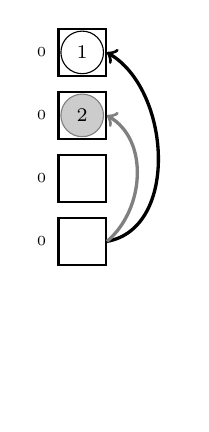
\begin{tikzpicture}
[
textbox/.style={rectangle, draw=white, fill=white,align=center, thick, minimum height=0.5cm},
box1/.style={rectangle, draw=black, fill=white, thick, minimum height=0.6cm, minimum width=2.4cm},
box2/.style={rectangle, draw=black, fill=white, thick, minimum height=0.6cm, minimum width=1.2cm},
box3/.style={rectangle, draw=black, fill=white, thick, minimum height=0.6cm, minimum width=0.6cm},
myarrow1/.style={single arrow, draw=black, fill=black, 
      minimum width = 1mm, single arrow head extend=1mm,
      minimum height=1cm},
myarrow2/.style={single arrow, draw=red, fill=red, 
      minimum width = 1mm, single arrow head extend=1mm,
      minimum height=1.3cm},
myarrow3/.style={single arrow, draw=blue, fill=blue, 
minimum width = 0.09cm, single arrow head extend=0.05cm,
minimum height=0.7cm},
mylabels/.style={text=black, font=\scriptsize},
    every label/.append style={mylabels},
greenball/.style={circle, draw=gray, fill=gray!40, minimum size=1mm},
redball/.style={circle, draw=black, fill=white, minimum size=1mm},
blueball/.style={circle, draw=gray, fill=gray, minimum size=1mm},
]

\node at (0,0) [box3,label={west:$\OLDEST_0$}] (b1)     {};
\node at (0,0) [redball] (g1) {{\scriptsize 1}};
\node at (0,-0.8) [box3,label={west:$\OLDER_0$}] (b2)      {};
\node at (0,-0.8) [greenball] (g2) {{\scriptsize 2}};
\node at (0,-1.6) [box3,label={west:$\OLD_0$}] (b3)               {};
\node at (0,-2.4) [box3,label={west:$\NEW_0$}] (b4)               {};
\node[scale=0.6] at (0.45,-4.3) [textbox] (omap1) {};
\draw [->,black, very thick] (b4.east) to [out=10,in=330] (b1.east) ;
\draw [->,gray,very thick] (b4.east) to [out=40,in=330] (b2.east) ;
\end{tikzpicture}
%\caption{}
\end{subfigure}
\begin{subfigure}[t]{0.3\textwidth} %two
\centering
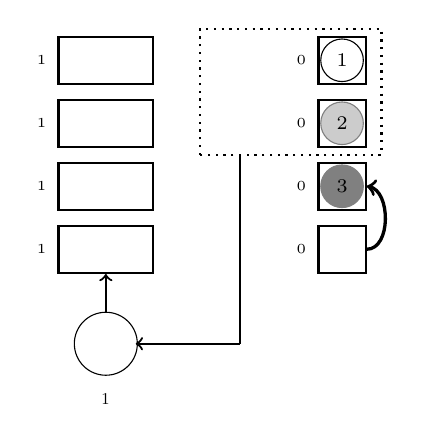
\begin{tikzpicture}
[
textbox/.style={rectangle, draw=white, fill=white,align=center, thick, minimum height=0.5cm},
box1/.style={rectangle, draw=black, fill=white, thick, minimum height=0.6cm, minimum width=2.4cm},
box2/.style={rectangle, draw=black, fill=white, thick, minimum height=0.6cm, minimum width=1.2cm},
box3/.style={rectangle, draw=black, fill=white, thick, minimum height=0.6cm, minimum width=0.6cm},
buf/.style={rectangle, draw=black, fill=white, very thick, minimum height=0.6cm, minimum width=1.2cm},
myarrow1/.style={single arrow, draw=black, fill=black, 
      minimum width = 1mm, single arrow head extend=1mm,
      minimum height=1cm},
myarrow2/.style={single arrow, draw=black, fill=red, 
      minimum width = 1mm, single arrow head extend=1mm,
      minimum height=1.3cm},
myarrow3/.style={single arrow, draw=blue, fill=blue, 
minimum width = 0.09cm, single arrow head extend=0.05cm,
minimum height=0.7cm},
mylabels/.style={text=black, font=\scriptsize},
    every label/.append style={mylabels},
    greenball/.style={circle, draw=gray, fill=gray!40, minimum size=1mm},
redball/.style={circle, draw=black, fill=white, minimum size=1mm},
blueball/.style={circle, draw=gray, fill=gray, minimum size=1mm},
]
\node at (0,0) [box2,label={west:$\OLDEST_1$}] (b10)  {};
\node at (0,-0.8) [box2,label={west:$\OLDER_1$}] (b11)   {};
\node at (0,-1.6) [box2,label={west:$\OLD_1$}] (b12)  {};
\node at (0,-2.4) [box2,label={west:$\NEW_1$}] (b13)  {};


\node[scale=0.6] at (0,-4.3) [textbox] (omap1) {\Large{$\omerge_1$}};
\draw[] (0,-3.6) circle (4mm) node (c2)  {};
\draw[color=black,thick,->]  (0,-3.2) -- (b13) {};
\draw[color=black,thick] (1.7,-1.2) -- (1.7,-3.6) {};
\draw[color=black,thick,->]  (1.7,-3.6) -- (0.38,-3.6) {};
\node at (3,0) [box3,label={west:$\OLDEST_0$}] (b10) {};
\node at (3,-0.8) [box3,label={west:$\OLDER_0$}] (b11)  {};
\node at (3,0) [redball] (g1) {{\scriptsize 1}};
\node at (3,-1.6) [box3,label={west:$\OLD_0$}] (b12)  {};
\node at (3,-0.8) [greenball] (g2) {{\scriptsize 2}};
\node at (3,-2.4) [box3,label={west:$\NEW_0$}] (b13)  {};
\node at (3,-1.6) [blueball] (g2) {{\scriptsize 3}};
\draw[dotted,color=black,thick] (1.2,-1.2) rectangle (3.5,0.4);
\draw [->,color=black!50!black,very thick] (b13.east) to [out=0,in=-10] (b12.east) ;
\end{tikzpicture}
%\caption{}
\end{subfigure}
}
%\caption{\LSDd[$\cdot$]: from $\Sigma$ to DSE.(a) Insertion of the 1st entry happens at $\NEW_0$(Rule 1), making $\NEW_0$ full. Hence it is moved to the empty old index $\OLDEST_0$ (Rule 2, red arrow). The 2nd insertion happens at $\NEW_0$ (Rule 1), making it full again, and is moved to next empty old index $\OLDER_0$ (Rule 2, dark red arrow).(b) During the 3rd insertion, both $\OLDEST_0$ and $\OLDER_0$ are full, so the next $\gamma$ steps of $\Sigma.$\omerge$_1$\ is called (Rule 3), moving entries from $\OLDEST_0\cup \OLDER_1$ (directly or via a buffer) to $\NEW_0$ in the next $2^1$ steps. The 3rd entry is inserted at $\NEW_0$ and moved to $\OLD_0$ (triggering Rule 1 and 2 respectively). (c) During the 4th insertion, $\OLDEST_0$ and $\OLDER_0$ are still full, hence next $\gamma$ steps of $\Sigma.$\omerge (Rule 3) is called. At this point $2^1$ steps of \omerge$_1$\ are done and $\NEW_1$ is full with entries of $\OLDEST_0\cup \OLDER_1$, and is moved to $\OLDEST_1$ (Rule 2, light red arrow). The 4th insertion causes $\NEW_0$ to be full. Hence $\OLD_0$ is moved to $\OLDEST_0$ (red arrow), and $\NEW_0$ is moved to $\OLDER_0$(dark red arrow).}
\label{fig:sddFig}
\end{figure}
	

\begin{figure*}[!h]
\begin{mdframed}
\begin{algorithmic}%[1]
 \Statex \hskip-1.5em$\Gamma \in \{\OneChoice,\TwoChoice, \NlogN \}$
\Statex \hskip-1.5em If $\Gamma = \OneChoice$, $N'= 3{\cdot} 2^i,m_i = \lceil{\frac{2^i}{\log 2^i \log \log 2^i}}\rceil$,  $\forall level\in \{0 \ldots m_i-1\}$ $b_{level} = 3{\cdot}\log 2^i\log \log 2^i$ and $c_{level} = 0$
\Statex \hskip-1.5em If $\Gamma = \NlogN$, $N'= 2^i{\cdot}\log{(2^i+1)}$, $m_i = (i+1)$,   $\forall level\in \{0 \ldots m_i-1\}$ $b_{level} = 2^{level}$ and $c_{level} = 2^{i-level}$
\Statex \hskip-1.5em If $\Gamma = \TwoChoice$, $N'= z{\cdot} 2^i,m_i = \lceil{\frac{2^i}{(\log \log 2^i) (\log \log \log 2^i)^2}}\rceil$,
$\forall level\in \{0 \ldots m_i-1\}$ $b_{level} = z{\cdot}(\log \log 2^i)(\log \log \log 2^i)^2$ and $c_{level} = 0$, $2 \leq z \leq 4$
\Statex
\end{algorithmic}
\underline {{${\sf NEW}_i$ $ \leftrightarrow$ {$\Gamma$.\omerge$_i(K, \sigma; {\sf OLDEST}_{i - 1},{\sf OLDER}_{i - 1})$}}}
\begin{algorithmic}[1]
\item[Client $\leftrightarrow$ Server:] %\tpurp{$\Gamma$ s inside the function should be deleted}
\Statex
\Statex \textcolor{blue}{//** \ \ Phase 1 - Preparing sorted input array\ \   **//}	
\State Client parses $K$ as $(k_{rnd},P)$ \label{fw:parseK}\Comment{all encryptions and decryptions are done with key $k_{rnd}$, $P$ is an array of PRF keys}
%\State Client initializes a tuple called $\pr$ as $(\bot, 0)$ and stores it in local state $\sigma$
\State {Server initializes} arrays \BUF$_1$ of size $3{\cdot}N'$, and \BUF$_2$ of size $N'$ to be empty at Server\label{fw:init}
%\State Perform oblivious sort on $\OLDEST_{i-1}.\Ind \cup \OLDER_{i-1}.\Ind$ in 
%the lexicographic order of keywords; store output in $\BUF_1$ \label{fw:firstsort}
\State Copy $\OLDEST_{i-1}.\Ind \cup \OLDER_{i-1}.\Ind$ to $\BUF_1$; obliviously sort $\BUF_1$ w.r.t. 
 lexicographic order of keywords\label{fw:firstsort}
\State Perform two linear scans (one in reverse and one in correct order) on $\BUF_1$, to add the $rank$ and $n_w$ values to each entry of keyword $w$. The entries now look like $(w,id,op,rank,n_w)$, where $0 \leq rank < n_w$. \label{fw:twoscans}
\State {Linearly scan $\BUF_1$ and pad each keyword-list with dummy elements so that its size is nearest power of 2, hide list lengths by padding total size to $2N'$}\label{fw:pad2}% without leaking the actual list length}
   % \State {$cnt \gets 0$}
   \State {Perform oblivious sort on $\BUF_1$ w.r.t. lexicographic order of the keywords and descending order of the $n_w$ values. Keep first $N'$ elements.}\label{fw:secondsort}
   \Statex
  \Statex \textcolor{blue}{//** \ \ Phase 2---Prepare index elements and prepare keyword counters \ \ **//}	
    \For{each $j = 1 \ldots |\BUF_1|$}\label{fw:loop1start}
    \State Client decrypts $(w,id,op,rank,n_w) \gets \RND.\Dec(k_{rnd},\BUF_1[j])$\label{fw:dec1} %
      \State Client generates {$p \gets^{\$} \{0,1\}^\lambda$}\label{fw:randp}
    \IIf{$rank = 0$}{~Client appends $(\RND.\Enc(k_{rnd},(w,n_w,p)))$ to $\BUF_2$}\label{fw:rank0} %\Comment{\tpurp{I want to do p+1 here}}
    \ElsI{Client appends $(\RND.\Enc(k_{rnd},(\bot,\bot,\bot)))$ to $\BUF_2$}\label{fw:rankN0}
    \State Client generates $((level,pos),\sigma)\gets\texttt{Map}(P[i][3],w,rank,n_w,\sigma)$\label{fw:map} \Comment{$pos=0$ for \OneChoice\ and \TwoChoice\ }
  \State Client writes $(\RND.\Enc(k_{rnd},(w,id,op,level,pos)))$ to \BUF$_{1}[j]$ \label{fw:dec2}
    \EndFor\label{fw:loop1end}
    \Statex
    \Statex \textcolor{blue}{//** \ \ Phase 3---Add dummies\ \ **//}	%\Comment{this phase adds binsize dummy entries per bin}
    \For{$level= 0 \ldots m_i-1$}\label{fw:loop2start}
    \State for every $pos \in\{0 \ldots c_{level}\}$ call Client appends $(\RND.\Enc(k_{rnd},(\bot,\bot,\bot,level,pos)))$ to $\BUF_1$  $b_{level}$ times \label{fw:padbin}
    \EndFor\label{fw:loop2end}
    \Statex
     \Statex \textcolor{blue}{//** \ \ Phase 4---Final placement \ \ **//}	
    \State Perform oblivious sort on $\BUF_1$ w.r.t. the integer values of $(level,pos)$ in ascending order \label{fw:thirdsort}
    \State Linearly scan $\BUF_1$, and tag \textbf{first} $b_{level}$ entries for each $level\in \{0, \ldots, \Sigma.m_i-1\}$ and $pos\in \{0, \ldots, c_{level}\}$ with 1, and with 0 the rest of them (the existing $(level,pos)$ tags are replaced with 0/1 tags, the entries now look like $(w,id,op,x)$, where $x \in \{0,1\}$)\label{fw:0-1tag}
    \State {Perform order preserving oblivious compaction on $\BUF_1$; keep first $N'$ entries; discard the 0/1 tags }\label{fw:compaction}
    \State Perform oblivious sort on $\BUF_2$ w.r.t. the random keys in ascending order; keep first $2^i$ entries; discard random keys\label{fw:buf2sort}
    \State 	Server moves $\BUF_1$ to \NEW$_i.\Ind$  \label{fw:newi} \Comment{elements in each $bin/pos$ is randomly shuffled}
   \For{each $s \in \BUF_2$}\label{fw:dictloopstart}
\State Client decrypts $(w, cnt_w) \gets \RND.\Dec(k_{rnd}, s)$\label{fw:dec3}
\State Client generates $(key,value) \gets \PiBas.\MAP((P[i][3],k_{rnd}),w,cnt_w,1)$ \label{fw:pibasmap}\Comment{parameter 1 is used by the PRF $F$}
\State 	Client writes \NEW$_i.$\Dict[$key$] $\gets value$\label{fw:mapdict}
\EndFor\label{fw:dictloopend}
%\Statex
\State \Return \NEW$_i$
\end{algorithmic}
\end{mdframed}
%\vspace{-1.2em}
\caption{\omerge\ framework of $\Gamma \in \{\OneChoice, \TwoChoice, \NlogN\}$}
\label{alg:framework}
\vspace{+1.3em}
\end{figure*}

\smallskip\noindent\textbf{Phases of {\omerge} framework.}\label{sec:oblivious_merge}
%\todo{5.Clearly explain that SDd[] works only with 1C/2C/NlogN and not scheme-agnostic}
Now we will present our \omerge\ framework that 
ensures properties \textsf{{(P1)}}, \textsf{{(P2)}}, 
and \textsf{{(P3)}} for the static 
SE scheme $\Gamma$ $\in$ $\{\OneChoice,$ $\TwoChoice,$ $\NlogN\}$, in detail. 
%\todo{7.Clarify which scheme targets which storage and which metrices} 
Similar to \SDa, we have \LSDd[\OneChoice] and \LSDd[\TwoChoice] (suitable for HDDs), as well as \LSDd[\NlogN] (compatible with both HDDs and SSDs).
The corresponding is presented in Figure \ref{alg:framework}. 
Some of the steps are not necessary for all the schemes in  $\{\OneChoice,$ $\TwoChoice,$ $\NlogN\}$, 
but we needed them in order to create the general \omerge\ framework. 
\new{Towards the end of this section we discuss some optimization specific to each scheme.  Here, we also would like to point out, the temporary client storage cost is upper bounded by the update cost (e.g. $\bO(\log^2 N)$ for \LSDd[\OneChoice]), while the permanent client storage is constant. }

The high level idea is, instead of moving elements directly from 
$\OLDER_{i-1}.\Ind \cup \OLDEST_{i-1}.\Ind$ to $\NEW_i.\Ind$ 
(using oblivious dictionaries, as done in \cite{SDa}), 
move them to a buffer $\BUF_1$ first. This step will ensure 
property \textsf{{(P2)}}. Then with oblivious operations, re-order the entries of $\BUF_1$ to 
satisfy the I/O efficiency requirements of scheme $\Gamma$, 
and then move $\BUF_1$ to $\NEW_i$.\Ind. {This step and the previous step 
together ensure property \textsf{{(P1)}}. 
{The buffer, $\BUF_2$, is used to create  
the keyword dictionary, $\NEW_i.\Dict$}, in an oblivious fashion as well.
The references to $\OLDER_{i-1}$ and $\OLDEST_{i-1}$ are passed as parameters to the \omerge$_i$ protocol.
Each \omerge$_i$ instance runs in four phases. Below we discuss the four phases in detail. Refer to Figure \ref{alg:framework} for the pseudocode. 
If a step in the pseudocode does not mention who is performing it (i.e. Client or Server), it means multiple rounds of communication happens between the client and the server to perform that step.}
\neww{Finally, at the end of $2^i$ calls to \omerge$_i$ it returns $\NEW_i$ (i.e. $\NEW_i.\Ind$  and $\NEW_i.\Dict$). }

\noindent\textbf{\underline{Phase 1.}} %In this phase 
\new{Entries of $\OLDER_{i-1}.\Ind \cup \OLDEST_{i-1}.\Ind$ are 
first copied (not moved) to $\BUF_1$.} Next, $\BUF_1$ is 
obliviously sorted based on the lexicographic order 
of the keywords (line \ref{fw:firstsort}). \new{The sort places 
entries for the same keyword adjacent to each other in $\BUF_1$, 
and the dummy entries are placed at the end. Each entry of 
$\BUF_1$ is then assigned a $rank$} and an $n_w$ value via two 
linear scans (line \ref{fw:twoscans}). Next, each keyword-list 
in $\BUF_1$ is padded to make their lengths to be nearest power of 2 
(line \ref{fw:pad2}). Another oblivious sort is performed on $\BUF_1$, 
based on the lexicographic order of the keywords, as well as descending 
order of the $n_w$ values   (line \ref{fw:secondsort}). This sort places 
same keyword entries adjacent to each other and entries with higher 
$n_w$ values are placed before entries with lower $n_w$ values in $\BUF_1$.

We provide a more detailed pseudocode for lines \ref{fw:twoscans} and \ref{fw:pad2} in the extended version.

\noindent\textbf{\underline{Phase 2.}} This phase prepares the elements in $\BUF_1$ for 
$\NEW_i.\Ind$ by adding proper position tags to them 
(lines \ref{fw:map}-\ref{fw:dec2}), and prepares $\BUF_2$ 
for creating $\NEW_i.\Dict$ (lines \ref{fw:randp}-\ref{fw:rankN0}). 
For every entry in $\BUF_1$\ $(w,id,op,rank,n_w)$ an entry is appended to 
$\BUF_2$. When $rank=0$, a real entry $(w,n_w,p)$ 
is appended to $\BUF_2$. 
\new{In all other cases a dummy entry $(\bot,\bot,\bot)$ is added (line \ref{fw:rankN0})
(because we can neither reveal the length of each keyword-list, nor the number of unique keywords). }
Here, $p$ is a uniformly generated random key of $\lambda$ bit.

The $\MAP$ function of $\Gamma$ is called for each 
entry of $\BUF_1$,  which %with appropriate arguments, which 
returns a pair $(level,pos)$. 

 \new{For every $\Gamma \in \{\OneChoice,\TwoChoice,\NlogN\}$ the pseudocode for the corresponding $\MAP$ function is provided in the extended version}.
For $\OneChoice$ and $\TwoChoice$ the value of $level$ indicates  
the bin number assigned to this entry, and $pos$ is 0 by default. 
Whereas, for \NlogN\ scheme 
$level(\in \{0,\ldots,i\})$ indicates the array level,
and position indicates the position $pos (\in \{0,\ldots, (2^{i-level}\minus1)\})$ in the array level.
The encrypted entry $(w,id,op,level,pos)$ replaces the existing 
$(w,id,op,rank,n_w)$ entry in $\BUF_1$. 

\noindent\textbf{\underline{Phase 3.}}
This phase adds dummy elements 
(lines \ref{fw:loop2start}-\ref{fw:loop2end}) to $\BUF_1$, beacuse  
every bin needs to be filled up to their maximum capacity. 
For \OneChoice\ and \TwoChoice\, if bin size is $b_i$ then 
the dummy element $(\bot,\bot,\bot,bin,0)$ is appended to $\BUF_1$ $b_i$ times. 
This step is repeated for each bin number $bin$.  
For \NlogN\ scheme, array level $k$ contains $2^{i-k}$ 
lists of size $2^k$.
Hence, the dummy entry $(\bot,\bot,\bot,k,pos)$ 
is appended $2^k$ times for each $pos \in \{0,\ldots, (2^{i-k}-1)\}$.
This step is repeated for levels $k \in \{0, \ldots, i\}$. 
\new{We add a total of $3{\cdot}2^i$ dummy elements for \OneChoice\ and 
\TwoChoice\, and $2^i{\cdot}\log {2^i}$ dummy elements for \NlogN.
The goal is to add dummy entries for every vacant positions of the bins/levels.
But we want} to hide the number of real elements {in each bin/level, and so 
 the number of dummy elements we add is equal to the index size.
Extra dummy elements are discarded in Phase 4.}
\noindent\textbf{\underline{Phase 4.}} 
This phase consists of few steps. 
%(lines \ref{fw:thirdsort}-\ref{fw:dictloopend}). 
%Each of them can be de-amortized.
The oblivious sort on line \ref{fw:thirdsort} 
sorts $\BUF_1$ based on $(level,pos)$ values.
Dummy elements come last, as usual.
But now we have more elements assigned to each bin/level than their capacity. 
Hence, with a linear scan (line \ref{fw:0-1tag}) 
unnecessary elements are tagged with a 0;
and the entries to be kept are tagged with a 1. 
%(red and blue tags respectively in Figure \ref{fig:buf1f}).
This tag replaces the existing $(level,pos)$ tags.
Next, an order preserving oblivious compaction (line \ref{fw:compaction}) is 
performed so that all elements tagged with 0 come at the tail of the output and 
can be discarded altogether. We use 
another round of oblivious bucket sort (which is order preserving) for the compaction. 
%The 0/1-bit tags are removed from each entry at the end.
%Next, the entries %at the beginning that were tagged with 
%1-bit in 
$\NEW_i.\Ind$ is created with the remaining entries of $\BUF_1$ (line \ref{fw:newi}). 
$\BUF_2$ is also obliviously sorted (line \ref{fw:buf2sort}) based on 
the random keys in ascending order. 
The dummy entries with $p=\bot$ will be placed at the end of the sorted buffer.
There can be at most $2^i$ entries such that $p \neq \bot$, as 
there can be at most $2^i$ distinct keywords at index level $i$.
Hence, the first $2^i$ elements are used to 
create $\NEW_i.\Dict$ (lines \ref{fw:dictloopstart}-\ref{fw:dictloopend}).

\smallskip\noindent\textbf{Locality-aware \LSDd$[\cdot]$.}
\new{The search-\emph{locality} and search-\emph{read efficiency} of \LSDd[$\Gamma$]
depends on the same of the static SE scheme $\Gamma$. For both \emph{locality} 
and \emph{read efficiency}, a $\log N$ factor is added 
due to querying $3{\cdot}\log N$ dictionaries and calling 
$\Gamma.\Search$ on $3{\cdot}\log N$ indexes (for \OLDEST, \OLDER, and \OLD). 
For example, \OneChoice\ offers $\bO(1)$ \emph{locality} 
and $\bO(\log N \log \log N)$ \emph{read efficiency}, whereas \LSDd[\OneChoice] offers 
$\bO(\log N)$ \emph{locality} and $\bO(\log N \log \log N +\log N)$ \emph{read efficiency}. 
Similarly, \LSDd[\NlogN] offers $\bO(\log N)$ \emph{locality} and $\bO(\log N)$ \emph{read efficiency}, 
as opposed to optimal \emph{locality} and \emph{read-efficiency} that is offered by \NlogN.} 

\smallskip\noindent\textbf{Page-efficient \LSDd{[.]}.}
We can instantiate \LSDd[$\cdot$] on SSDs with static page efficient schemes 
like \NlogN\  \cite{onechoice} and its variations i.e. \Ns\ \cite{Demertzis17}. 
The \emph{page efficiency} of \LSDd[\NlogN] is $\bO(\log N)$ vs. the 
optimal \emph{page efficiency} offered by \NlogN, whereas 
for \LSDd[\Ns] \emph{page efficiency} is $\bO(N^{\frac{1}{s}}/p+\log N)$. 

\smallskip\noindent\textbf{Security and efficiency.} We formally state and prove the security of \LSDd[$\Gamma$] 
(for $\Gamma \in \{\OneChoice,\TwoChoice,\NlogN\}$) in the extended version. The security of \SDd[\PiBas] is already proven in \cite{SDa}. 
We prove also that when we instantiate a locality-aware static scheme $\Gamma$ with \LSDd[$\cdot$], it retains its space overhead, but for \emph{locality} and \emph{read-efficiency} an additional $3\log N$ factor is introduced as $3\log N$ indexes are queried (similar proof for the \emph{page-efficient} \LSDd[$\cdot$] transformation can be proven)---see the extended version. 

\smallskip\noindent\textbf{\OneChoice\ Optimization.} 
In \OneChoice\ scheme we do not need to make the keyword-lists' sizes to be of power of 2. 
We also do not need to store the larger keyword-lists into the bins before the 
smaller lists. Hence the lines \ref{fw:pad2} and \ref{fw:secondsort} 
in Figure \ref{alg:framework} are not required for \OneChoice.
%In Figure \ref{alg:sdd1C} those two lines are omitted.
The two linear scans that add $rank$ and
$n_w$ values to each entry can be also removed (line \ref{fw:twoscans}). 
This is because, after the first oblivious sort
the entries for the same keyword are all placed together in adjacent locations. In Phase 2, with the help of a single counter 
%($cnt$ variable in 
%line \ref{sdd1c:counter} in Figure \ref{alg:sdd1C}), 
one can count how many occurrences of 
a particular keyword has been seen. %(and $\BUF_2$ can be updated accordingly).
Based on this counter value $\BUF_2$ can be updated accordingly.
The same counter value can be used in $\OneChoice.\MAP$ function to compute 
the bin numbers.% (line \ref{sdd1c:map} in Figure \ref{alg:sdd1C}).
The counter needs to be reset to 0 every time a new keyword is observed. We provide the optimized pseudocode for  \OneChoice.\omerge\ in the extended version. 


\smallskip\noindent\textbf{\NlogN\ Optimization.} 
%\paragraph{{\textbf{\NlogN\ Optimization.}}}
Here the order of storing lists does not matter.
Thus, the second oblivious sort (line \ref{fw:secondsort}) can be omitted in Phase 1 for the \NlogN\ scheme.
This can be further optimized 
by storing only $s$ evenly distributed arrays, 
instead of $\ell=\log N+1$ arrays, which 
is essentially the \textsf{Ns} scheme.

\smallskip\noindent\textbf{\TwoChoice\ Optimization.} 
For \TwoChoice\ scheme, the client needs to maintain a map to remember which bin has how many entries.
This is because, placement of a keyword-list into a superbin 
depends on how full the superbin is. 
There are can be maximum of $m = \lceil{{N}/{\log\log N (\log \log \log N)^2}}\rceil$  
bins. But in \LSDd\ there are $\log N$
index levels. Hence, to maintain this information the required  
client storage is $\bO(m{\cdot}\log N)$.
To achieve a constant client storage, this map can 
be stored at the server in oblivious maps (see section \ref{sec:prelim}).

\smallskip\noindent\textbf{Update cost.}
The \omerge\ framework shown in Figure \ref{alg:framework} mainly consists of three types of building blocks: bucket oblivious sorts, 
basic \algorithmicfor\ loops and linear scans.
Linear scans are realized with basic \algorithmicfor\ loops. 
The costliest operation among these is the bucket oblivious sort \cite{bucketSort}, 
which can be decomposed into $N$ steps of $\bO(\log N)$ work per step, 
assuming an index contains at most $N$ entries 
(recall the $i$th index contains $2^i$ elements).
In the extended version we explain how to 
deamortize the bucket oblivious sort in detail. 
Even the \algorithmicfor\ loops can be executed for $\bO(\log N)$ 
iterations during a particular call of \omerge$_i$ (for the $i$th index). Overall, an \omerge$_{i}$ protocol can be decomposed into $N$ steps of at most $\bO(\log N)$ work per step. There are $\log N$ levels in \LSDd[${\cdot}$]. Hence, the \emph{worst case} update cost is $\bO(\log^2 N)$ for \LSDd[\OneChoice], and \LSDd[\TwoChoice]. For \LSDd[\NlogN] the update cost is $\bO(\log^3 N)$, because it has at most $\log N$ levels per index.
%\section{Experimental Evaluation}\label{sec:eval}

\begin{figure}[t]
\small
 \centering\begin{tabular}{|c|c|c|} 
\hline
\multirow{2}{*}{\parbox{2cm}{\centering Scheme}} & \multirow{2}{*}{\parbox{2cm}{\centering Size(GB) for $|DB|=2^{23}$}} & \multirow{2}{*}{\parbox{2cm}{\centering Size(GB) for $|DB|=2^{26}$}} \\ & & \\
\hline 
 \LSDd[\NlogN] & 49 & 436 \\
 \LSDd[\OneChoice] & 7.5 & 60\\
 \SDd[\PiBas] & 5 & 40 \\
\hline
\end{tabular}
%\end{adjustbox}
\caption{Needed storage for a dataset and encrypted index.}
\label{table:storage}
\end{figure} 
%\tgreen{ I/O matters for in memory too.}
%\tgreen{ Repository link of the code}
%\tgreen{why SDd[Pibas] better that SDa[PiBas] in some cases}.
We report the performance of our schemes and compare them with previous state-of-the-art works. 
\begin{figure*}[ht]
	\centering
	\begin{subfigure}[t]{0.24\linewidth}
		\includegraphics[width=\textwidth]{chapters/iodse/figures/Search-Comp-DBSize10M-ResultSizeVar-32B-NoCache.eps}
		\vspace{-0.8cm}
		\caption{}
	\end{subfigure}
 	\begin{subfigure}[t]{0.24\linewidth}
		\includegraphics[width=\textwidth]{chapters/iodse/figures/Search-Comp-DBSize10M-ResultSizeVar-32B-NoCache-SSD.eps}
		\vspace{-0.8cm}
		\caption{}
	\end{subfigure}
		\begin{subfigure}[t]{0.24\linewidth}
		\includegraphics[width=\textwidth]{chapters/iodse/figures/Search-Comp-DBSizeVar-ResultSize1000.eps}
		\vspace{-.8cm}
		\caption{}
	\end{subfigure}
 	\begin{subfigure}[t]{0.24\linewidth}
		\includegraphics[width=\textwidth]{chapters/iodse/figures/Search-Comp-DBSizeVar-ResultSize1000-SSD.eps}
		\vspace{-.8cm}
		\caption{}
	\end{subfigure}%

	\vspace{-.3cm}
	\caption{Search computation time for $|{DB}|=2^{23}$ and variable result size for (a) $|block|=32$B in (a) HDD, (b) SSD. Search computation time for variable database size and $n_w=1K$ in (c) HDD, (d) SSD.}
	\label{fig:search-var}
	%\vspace{-.5em}
\end{figure*}

\begin{figure*}[ht]
	\centering
	\begin{subfigure}[t]{0.24\linewidth}
		\includegraphics[width=\textwidth]{chapters/iodse/figures/Search-Comp-DBSize10M-ResultSizeVar-512B-NoCache.eps}
		\vspace{-.8cm}
		\caption{}
	\end{subfigure}%
 	\begin{subfigure}[t]{0.24\linewidth}
		\includegraphics[width=\textwidth]{chapters/iodse/figures/Search-Comp-DBSizeVar-ResultSize10000.eps}
		\vspace{-.8cm}
		\caption{}
	\end{subfigure}~
		\begin{subfigure}[t]{0.24\linewidth}
		\includegraphics[width=\textwidth]{chapters/iodse/figures/Search-Comp-DBSizeVar-ResultSize10000-SSD.eps}
		\vspace{-.8cm}
		\caption{}
	\end{subfigure}~
  \begin{subfigure}[t]{0.24\linewidth}
		\includegraphics[width=\textwidth]{chapters/iodse/figures/SearchTime-WAN2.eps}
		\vspace{-0.6cm}
	\end{subfigure}\\
	%\vspace{-.3cm}
	\caption{Search computation time for $|{DB}|=2^{23}$ and variable result size for (a)  $|block|=512$B in HDD. Search computation time for variable database size and $n_w=10K$ in (b) HDD, (c) SSD. (d) Search computation time for $|{DB}|=2^{23}$, $|block|=32$B in HDD and variable result size for WAN machines with 24.7ms network delay and 2.5Gbps bandwidth.}
	\label{app-fig:search-var2}
% 	\vspace{-.3cm}
\end{figure*}

We implemented \SDa[\OneChoice], \SDa[\TwoChoice], \SDa[\NlogN], \SDa[\textsf{\Ns}], \LSDd[\OneChoice] and \LSDd[\sN] with approximately 
$31K$ lines in C++. 
We used  OpenSSL-AES~\cite{openssl} 
PRF evaluation and semantically secure encryption. 
We also used Oblivious MAP of~\cite{SDa} {for the \SDd[\PiBas] implementation}, 
and merge-sort as the last step in the implementation of 
bucket oblivious sort~\cite{bucketSort}. We ran our experiments on a machine with
%\tgreen{highlight single core implementation} 
Intel Xeon E-2174G 3.8GHz processor,  128GB  RAM, 1TB SSD, and 5TB HDD running 
Ubuntu 20.04 LTS (limited to one CPU core for our experiments). 
%All schemes were instantiated on a single machine, \tpurp{although communication time between a client and a server can be easily simulated}. 
Our code is available online.\footnote{https://github.com/jgharehchamani/DSE-with-IO-Locality} %\tgreen{SSD/HDD speeds/ RAM speed DDRx ?}







\begin{figure*}[ht]
	\centering
	\begin{subfigure}[t]{0.24\linewidth}
		\includegraphics[width=\textwidth]{chapters/iodse/figures/Search-Comp-DBSize10M-ResultSizeVar-32B-NoCache-2.eps}
		\vspace{-0.8cm}
		\caption{}
	\end{subfigure}
	\begin{subfigure}[t]{0.24\linewidth}
		\includegraphics[width=\textwidth]{chapters/iodse/figures/Search-Comp-DBSize10M-ResultSizeVar-512B-NoCache-2.eps}
		\vspace{-.8cm}
		\caption{}
	\end{subfigure}%
		\begin{subfigure}[t]{0.24\linewidth}
		\includegraphics[width=\textwidth]{chapters/iodse/figures/Search-Comp-DBSizeVar-ResultSize1000-2.eps}
		\vspace{-.8cm}
		\caption{}
	\end{subfigure}~
 	\begin{subfigure}[t]{0.24\linewidth}
		\includegraphics[width=\textwidth]{chapters/iodse/figures/Search-Comp-DBSizeVar-ResultSize10000-2.eps}
		\vspace{-.8cm}
		\caption{}
	\end{subfigure}~\\
% 	\vspace{-.4cm}
% 	\caption{Search computation time for $|{DB}|=2^{23}$ and variable result size for: (a) $|block|=32$B in HDD, (a) $|block|=32$B in SSD, (c) $|block|=512$B in HDD.}
% 	\label{fig:search-var-block}
	\vspace{-.2cm}
% \end{figure*}

% \begin{figure*}[ht]
% 	\centering
	\begin{subfigure}[t]{0.24\linewidth}
		\includegraphics[width=\textwidth]{chapters/iodse/figures/Search-Comp-DBSize10M-ResultSizeVar-32B-NoCache-SSD-2.eps}
		\vspace{-0.8cm}
		\caption{}
	\end{subfigure}
	\begin{subfigure}[t]{0.24\linewidth}
		\includegraphics[width=\textwidth]{chapters/iodse/figures/Search-Comp-DBSizeVar-ResultSize1000-SSD-2.eps}
		\vspace{-.8cm}
		\caption{}
	\end{subfigure}%
		\begin{subfigure}[t]{0.24\linewidth}
		\includegraphics[width=\textwidth]{chapters/iodse/figures/Search-Comp-DBSizeVar-ResultSize10000-SSD-2.eps}
		\vspace{-.8cm}
		\caption{}
	\end{subfigure}~
	\vspace{-.3cm}
	\caption{Search computation time for $|{DB}|=2^{23}$ and variable result size for (a) $|block|=32$B in HDD, (b) $|block|=512$B in HDD. Search computation time for variable database size and (c) $n_w=1K$ in HDD, (d) $n_w=10K$ in HDD. Search computation time for $|{DB}|=2^{23}$ and variable result size for (e) $|block|=32$B in SSD. Search computation time for variable database size and (f) $n_w=1K$ in SSD, (g) $n_w=10K$ in SSD.}
	\label{app-fig:search-var}
% 	\vspace{-.3cm}
\end{figure*}

\begin{figure}[!ht]
	\centering
	\begin{subfigure}[t]{0.49\linewidth}
		\includegraphics[width=\textwidth]{chapters/iodse/figures/Search-SDA.eps}
		\vspace{-0.8cm}
		\caption{}
	\end{subfigure}
	\begin{subfigure}[t]{0.49\linewidth}
		\includegraphics[width=\textwidth]{chapters/iodse/figures/Search-SDA-SSD.eps}
		\vspace{-.8cm}
		\caption{}
	\end{subfigure}%
	\vspace{-.3cm}
	\caption{Search computation time for $|{DB}|=2^{23}$, variable result size, and $|block|=32$B for different \NlogN settings in (a) amortized HDD, (b) amortized SSD.}
	\label{app-fig:search-var-amor-deamor}
% 	\vspace{-.3cm}
\end{figure}

% \begin{figure*}[ht]
% 	\centering
% 	\begin{subfigure}[t]{0.33\linewidth}
% 		\includegraphics[width=\textwidth]{figures/Search-Comp-DBSize10M-ResultSizeVar-32B-NoCache.eps}
% % 		\vspace{-0.8cm}
% 		\caption{}
% 	\end{subfigure}
% 	\begin{subfigure}[t]{0.33\linewidth}
% 		\includegraphics[width=\textwidth]{figures/Search-Comp-DBSize10M-ResultSizeVar-32B-NoCache-SSD.eps}
% % 		\vspace{-.8cm}
% 		\caption{}
% 	\end{subfigure}%
% 		\begin{subfigure}[t]{0.33\linewidth}
% 		\includegraphics[width=\textwidth]{figures/Search-Comp-DBSize10M-ResultSizeVar-512B-NoCache.eps}
% % 		\vspace{-.8cm}
% 		\caption{}
% 	\end{subfigure}~
% % 	\vspace{-.4cm}
% 	\caption{Search computation time for $|{DB}|=2^{23}$ and variable result size for: (a) $|block|=32$B in HDD, (a) $|block|=32$B in SSD, (c) $|block|=512$B in HDD.}
% 	\label{fig:search-var-block}
% % 	\vspace{-.3cm}
% \end{figure*}

% \begin{figure*}[ht]
% 	\centering
% 	\begin{subfigure}[t]{0.24\linewidth}
% 		\includegraphics[width=\textwidth]{figures/Search-Comp-DBSizeVar-ResultSize1000.eps}
% % 		\vspace{-0.8cm}
% 		\caption{}
% 	\end{subfigure}
% 	\begin{subfigure}[t]{0.24\linewidth}
% 		\includegraphics[width=\textwidth]{figures/Search-Comp-DBSizeVar-ResultSize1000-SSD.eps}
% % 		\vspace{-.8cm}
% 		\caption{}
% 	\end{subfigure}%
% 		\begin{subfigure}[t]{0.24\linewidth}
% 		\includegraphics[width=\textwidth]{figures/Search-Comp-DBSizeVar-ResultSize10000.eps}
% % 		\vspace{-.8cm}
% 		\caption{}
% 	\end{subfigure}~
% 	\begin{subfigure}[t]{0.24\linewidth}
% 		\includegraphics[width=\textwidth]{figures/Search-Comp-DBSizeVar-ResultSize10000-SSD.eps}
% % 		\vspace{-.8cm}
% 		\caption{}
% 	\end{subfigure}%
% % 	\vspace{-.4cm}
% 	\caption{Search computation time for variable database size and (a) $|result|=1K$ in HDD, (b) $|result|=1K$ in SSD, (c) $|result|=10K$ in HDD, (d) $|result|=10K$ in SSD}
% 	\label{fig:search-var-db}
% % 	\vspace{-.3cm}
% \end{figure*}
We focus on the computation time for Search and Update queries and measure these parameters for variable-size synthetic datasets with $|{DB}| = 2^{11}$-$2^{26}$ records randomly shuffled before insertion, each time setting the total number of distinct keywords $|W|$ to $|{DB}|/100$. Likewise, we report results for varying result size $n_w$ between $10$ and $5M$ documents. We also consider two block sizes: 32B and 512B. %\tgreen{why this two blocksize only} 
%To demonstrate the importance of I/O in environment with limited available memory, we perform the experiments in a cold cache environment. 
\neww{To highlight the significance of I/O in a memory-constrained environment, we conduct our experiments in a cold cache setting, but we also provide two sets of experiments to show the effect of cache on the performance of our schemes. In the first one, we keep the different ratios of datasets in the memory (as cache) and respond to the queries for those encrypted data from memory. Note that we normalize the cache for each scheme. In other words, we fix the cache size and load as much as data we can in that memory.}
% Clearly, schemes with more storage need can benefit less from the cache. 
\neww{In the second, we assume there are many users ($200$ for HDD and $75$ for SSD) each of which has her own dataset with size $2^{20}$ and they execute their own search queries randomly when the cache in the system is enabled.}
%To demonstrate the effect of locality on the execution time, we disabled the hard-disk caching mechanism using \path{hdparm} and \path{nvme} commands and dropped the operating system's cache before each disk access by writing to \path{/proc/sys/vm/drop_caches}. 

Experiments were repeated five times, and the average result is reported. \neww{We also provide a comparison between the needed storage on the server for each de-amortized scheme in Figure~\ref{table:storage} for a dataset with $|block|=32B$ where $|DB|=2^{23}$ and $|DB|=2^{26}$. Note that we focus on small client storage schemes. Therefore, client storage is constant.}




%
% In addition to computation time, we compared the used storage of our schemes with the previous works (see Table~\ref{table:storage}). We measured this for a dataset with size $2^{23}-1$ (to fill all levels of the amortized schemes) and a block size of 32 bytes. For \SDd[\PiBas] scheme, the OMAP storage is also counted in the needed storage.
We also repeated the search experiments on a real dataset  consisting of $22$ attributes and $6,123,276$ records of reported crime incidents in Chicago~\cite{crimes}. We used two different attributes, containing 34 and 170 distinct keywords, respectively, and keyword frequency ranging from $1$ record to $1,631,721$ records.
\neww{Finally, we simulated the search and update time of our schemes when run over WAN with 24.7ms delay and 2.5Gbps bandwidth on AWS (between two machines on Ireland and Frankfurt zones).}

\subsection{Search Performance}
Our first set of experiments focuses on search performance and we demonstrate the impact of variable data block sizes, variable result sizes, variable database sizes, \neww{and cache size on all our schemes and compare them with \SDa[\PiBas]~\cite{SDa} and \SDd[\PiBas]~\cite{SDa}. We do not provide the big-block experiments for SSD due to disk space limits.}
%\todo{15. Explain if experimental results can be reproduced in more realistic settings}

\smallskip\noindent\textbf{Variable Block and Result Sizes.} Figure~\ref{fig:search-var} (a,b) and  Figure~\ref{app-fig:search-var2} (a) show the search computation time of a dataset with size $2^{23}$  $|block|=32$B as the result size $n_w$ changes. Similar results for our amortized schemes are in Figure~\ref{app-fig:search-var} (a),(b),(e).

% (results for $|block|=512$B are in Appendices~\ref{append:perf-amort} and~\ref{append:perf-deamort}. 
% a
% nd \ref{}). 
The  conclusions from these experiments are: 
(i) As expected, \SDa[\PiBas] and \SDd[\PiBas]\ have the worst performance among all other schemes for large result sizes due to their poor locality (in HDD) and page efficiency (in SSD). They need to change the position of the hard-drive head or bring different pages of the results, stored at random locations, which leads to significant {slowdown}. (ii) The \SDa[\NlogN]\ and \LSDd[\NlogN] schemes achieve the best performance in the amortized and de-amortized setting, at the cost of extra storage. The number of indexes searched in \LSDd[$\cdot$] is three times than that of \SDa[$\cdot$], hence the search time of \LSDd[\NlogN] is slightly 
more than \SDa[\NlogN]. (iii) \SDa[\TwoChoice] performs better than \SDa[\OneChoice] for small result sizes. However, their performance is the same for result sizes more than the bin's threshold, since, after the threshold entries are stored using \SDa[\OneChoice] (therefore we ignored this scheme in SSD experiments). (iv) The execution time for \SDa[\OneChoice] for result sizes bigger than $10^5$ remains approximately constant, as at this point the database is read in its entirety (i.e. all bins contain results). (v) When the block size is increased from 32B to 512B, 
the search time of all schemes increases, but the gap between \SDa[\TwoChoice]/\SDa[\OneChoice] and \SDa[\PiBas] decreases. This is due to the increase in the volume of the data read for blocks of size 512B, which becomes the dominant factor in the performance. (vi) Amortized and de-amortized versions of \PiBas, \OneChoice, and \NlogN\ have similar performance.
Finally, all our schemes have excellent performance in practice. E.g., \SDa[\OneChoice] and \SDa[\NlogN]/\LSDd[\NlogN] are up to three orders of magnitude faster than \SDa[\PiBas]/\SDd[\PiBas] (for $|n_w|=10^5$ and $|DB|=2^{23}$ \SDa[\OneChoice], \SDa[\NlogN], and \SDa[\PiBas] take 16s, 0.8s, and 903s respectively).

% \todo{26.Explain how communication cost and latency is improved in our scheme}
% \todo{27.Explain Why fully disabling HDD caching the right evaluation point }
% \todo{28. Experiments with client and server on separate machines}
% \todo{33. Provide sizes of the databases in bytes(NDSS)}
% \todo{34.”Real impact of HDD/SDD speeds unclear”(NDSS)}
% \todo{37. Evaluate performance on a larger database(NDSS)}



% \subsection{\SDa\textup{[\NlogN]} Update Experiment} \label{append:sda-nlogn}


\smallskip\noindent\textbf{Variable Database Size.} Figures~\ref{fig:search-var} (c,d) and Figures~\ref{app-fig:search-var2} (b),(c) show the effect of database size on search computation. (Results for the amortized schemes are in Figures~\ref{app-fig:search-var2} (c),(d),(f),(g)). For small blocks it varies search time for variable database sizes between $2^{11}-2^{26}$ and for result size $n_w$=1K in HDD and SSD. As the figures show, the search time of all schemes increases as the database size increases, because of the added levels in the data structures. However, all our schemes are significantly faster than \SDa[\PiBas] and \SDd[\PiBas]. For instance, the amortized schemes \SDa[\OneChoice], \SDa[\TwoChoice], and \SDa[\NlogN] are faster than \SDa[\PiBas] by $2-136\times$, $5-159\times$, and $4-209\times$ respectively. Also, the de-amortized schemes, \LSDd[\OneChoice] and \LSDd[\NlogN] are faster than \SDd[PiBAS] by $2-58\times$ and $3-70\times$ respectively.

\begin{figure*}[ht]
	\centering
	\begin{subfigure}[t]{0.24\linewidth}
		\includegraphics[width=\textwidth]{figures/Cache-25.eps}
		\vspace{-.8cm}
		\caption{}
	\end{subfigure}%
		\begin{subfigure}[t]{0.24\linewidth}
		\includegraphics[width=\textwidth]{figures/Cache-50.eps}
		\vspace{-.8cm}
		\caption{}
	\end{subfigure}~
 	\begin{subfigure}[t]{0.24\linewidth}
		\includegraphics[width=\textwidth]{figures/Cache-75.eps}
		\vspace{-.8cm}
		\caption{}
	\end{subfigure}
 	\begin{subfigure}[t]{0.24\linewidth}
		\includegraphics[width=\textwidth]{figures/Cache-100.eps}
		\vspace{-0.8cm}
		\caption{}
	\end{subfigure}~\\
	\vspace{-.4cm}
	\caption{Search computation time for $|{DB}|=2^{23}$ and variable result size for $|block|=32$B in HDD, (a) 25\% Caching, (b) 50\% Caching, (c) 75\% Caching, (d) 100\% Caching.}
	\label{fig:cache-hdd}
	%\vspace{-.2cm}
\end{figure*}
\begin{figure*}[ht]
	\centering
	\begin{subfigure}[t]{0.24\linewidth}
		\includegraphics[width=\textwidth]{chapters/iodse/figures/Cache-25-SSD.eps}
		\vspace{-.8cm}
		\caption{}
	\end{subfigure}%
		\begin{subfigure}[t]{0.24\linewidth}
		\includegraphics[width=\textwidth]{chapters/iodse/figures/Cache-50-SSD.eps}
		\vspace{-.8cm}
		\caption{}
	\end{subfigure}~
 	\begin{subfigure}[t]{0.24\linewidth}
		\includegraphics[width=\textwidth]{chapters/iodse/figures/Cache-75-SSD.eps}
		\vspace{-.8cm}
		\caption{}
	\end{subfigure}
    \begin{subfigure}[t]{0.24\linewidth}
		\includegraphics[width=\textwidth]{chapters/iodse/figures/Cache-100.eps}
		\vspace{-0.8cm}
		\caption{}
	\end{subfigure}~\\
	\vspace{-.4cm}
	\caption{Search computation time for $|{DB}|=2^{23}$ and variable result size for $|block|=32$B in SSD, (a) 25\% Caching, (b) 50\% Caching, (c) 75\% Caching, (d) 100\% Caching.}
	\label{fig:cache-ssd}
	%\vspace{-.2cm}
\end{figure*}

\begin{figure}[ht]
	\centering
	\begin{subfigure}[t]{0.48\linewidth}
		\includegraphics[width=\textwidth]{chapters/iodse/figures/email-hdd.eps}
		\vspace{-0.6cm}
		\caption{}
	\end{subfigure}
 \begin{subfigure}[t]{0.48\linewidth}
		\includegraphics[width=\textwidth]{chapters/iodse/figures/email-ssd.eps}
		\vspace{-0.6cm}
		\caption{}
	\end{subfigure}
	\vspace{-.3cm}
	\caption{Search computation time for $|{DB}|=2^{20}$ for each user and variable result size for $|block|=32$B with caching enabled in (a) HDD where 200 users exist in the system (b) SSD where 75 users exist in the system}
	\label{fig:email}
% 	\vspace{-.3cm}
\end{figure}






\smallskip\noindent\textbf{Effect of the value of \emph{s} on \SDa[\NlogN] and \LSDd[\NlogN].} The previous experiments showed that our \NlogN-based schemes have the best performance at a cost 
of more (i.e. $\log N$ times) storage.
% \footnote{For the vanilla \NlogN\ scheme the value of $s$ is $\log N$}. 
However, as discussed in Section ~\ref{sec:oblivious_merge}, these schemes can be used more "cleverly" to reduce the storage overhead. In Figure~\ref{fig:search-var} (a,b), we measured the effect of keeping $s$ intermediate levels instead $\log N$ levels for the de-amortized schemes (e.g., \LSDd[\textsf{3N}] refers to keeping 3 levels).  Similar experiments for amortized schemes are presented in Figure~\ref{app-fig:search-var-amor-deamor}. %We tried to store the entries at an existing level. 
If the level that a keyword-list should be stored does not exist, we split the 
list into multiple equal-sized chunks (last chunk is padded, if necessary) 
and store them in the next closest existing level. The experiment shows that even when keeping fewer levels than $\log N$, \SDa[\NlogN]/\LSDd[\NlogN] outperform \PiBas\ and \OneChoice\ based schemes in terms of search time, due to its practical locality and page efficiency, while also reducing storage to $3s\times N$. E.g., when storing every 8th level (\SDa[\textsf{3N}]/\LSDd[\textsf{3N}]), the achieved scheme is up to $30\times$ and $1949\times$ faster than \SDa[\OneChoice] and \SDa[\PiBas] and up to $8\times$ and $833\times$ faster than {\LSDd[\OneChoice]} and \LSDd[\PiBas] for big result sizes. 
% This comes from the fact that the \SDa[{\textsf{ Ns}]/\LSDd[\textsf{Ns}] scheme has better 
% Clearly, this also considerably reduces the needed storage, e.g., {storing only 3 levels results in $3\times N$ storage for \SDa[\textsf{3N}], 
% instead of $\log N \times N$.}
%Also, note that in J16 setting, the \NlogN\ performance becomes similar to \PiBas\ because the entries have to be split into lots of small size chunks, and finding each one of them would need a separate disk access (similar to \PiBas).  



\smallskip\noindent\textbf{Cache Experiment.}
 \neww{Figures~\ref{fig:cache-hdd} and \ref{fig:cache-ssd} show the effect of cache on the search time. They represent the search computation time over a dataset with size $2^{23}$ and $|block|=32B$ for variable result sizes and variable cache sizes on HDD (Figure~\ref{fig:cache-hdd}) and SSD (Figure~\ref{fig:cache-ssd}).
 % in Appendix~\ref{append:perf-deamort}). 
 As explained above, for these experiments we fix the cache size in memory according to the \SDd[\PiBas] scheme which has the smallest storage size in the de-amortized schemes (e.g., $25\%$ of the encrypted dataset of \SDd[\PiBas]), and we use the same cache size as for other schemes for fairness. The figures show that: i) as the cache size increases, all schemes' perform better and their search time reduces. However, \SDd[\PiBas] benefits more from the cache than others (i.e., its search time improves up to 8$\times$ while \LSDd[\OneChoice] and \LSDd[\NlogN] only improve up to $2.4\times$ and $2\times$) due to the smaller needed storage. ii) all our schemes still outperform \SDd[\PiBas] for big enough result sizes ($>$1K). Even when $75\%$ of data is cached in \SDd[\PiBas], \LSDd[\OneChoice] and \LSDd[\NlogN] are up to $191\times$ and $641\times$ faster. iii) When all data is cached (assuming it fits entirely in memory), \LSDd[\NlogN] outperforms other schemes (as expected) because it has the best locality and needs minimal cryptographic operations. On the other hand, \LSDd[\OneChoice] becomes worse than \SDd[\PiBas] in big result sizes because in these queries the dominant overhead comes from crypto and \LSDd[\OneChoice] needs to execute ${\sim}3\times$ more decryptions than the other schemes due to padding.}



\neww{In a second experiment (Fig.~\ref{fig:email})
% in Appendix~\ref{append:perf-deamort}) 
we emulate a scenario with multiple users ($200$ for HDD and $75$ for  SSD) each with her own independent dataset (of size $2^{20}$). With cache enabled, we executed random queries among users. As the figure shows, due to the size of datasets being larger than the memory (encrypted indexes for HDD and SSD were 1.8TB and 675GB), we see a similar trend as Figures~\ref{fig:search-var} (a, b).}


\begin{figure}[t]
	\centering
	\begin{subfigure}[t]{0.48\linewidth}
		\includegraphics[width=\textwidth]{chapters/iodse/figures/Search-Crime1.eps}
		\vspace{-0.8cm}
		\caption{}
	\end{subfigure}
	\begin{subfigure}[t]{0.48\linewidth}
		\includegraphics[width=\textwidth]{chapters/iodse/figures/Search-Crime2-2.pdf}
		\vspace{-.8cm}
		\caption{}
	\end{subfigure}%
	
	\vspace{-.3cm}
	\caption{Crime Dataset---Search computation time vs variable result size for an attributed with (a) $|W|=34$, (b) $|W|=170$.}
	\label{app-fig:real}
% 	\vspace{-.3cm}
\end{figure}


\smallskip\noindent\textbf{Search Over Real Datasets.}  We evaluated search times on two attributes of the crime dataset~\cite{crimes}, with (a) $34$, and (b) $170$ distinct keywords. We measured the search time for different keywords associated with increasing numbers of results. Our experiments show that our schemes clearly outperform both \SDa[\PiBas] and \LSDd[\PiBas], and we reach similar conclusions as previously (Figure~\ref{app-fig:real}). 



\smallskip\noindent\textbf{Search Over WAN}
\neww{We also simulated the end-to-end search time when client and server are located on two different machines. Our testbed was two AWS machines in Ireland and Frankfurt (with 24.7ms delay and 2.5Gbps bandwidth). Our experiments show a similar trend as the single machine case due to the constant roundtrip number and high network bandwidth, so our schemes outperform \SDa[\PiBas] and \SDd[\PiBas] (see Fig.~\ref{app-fig:search-var} (d)).}


\subsection{Update Performance}
Next, we report the update performance of our schemes via two sets of experiments: (i) update cost of the amortized scheme, (ii) update cost of the de-amortized schemes.

\smallskip\noindent\textbf{Update Cost of Amortized schemes.} In the first experiment, we measured the update time for 1K consecutive updates. Each time, the client fetches and merges some previously built levels and then uploads them to the server. Clearly, the update cost depends on the number of previously inserted indexes and it increases when more indexes need to be merged. We repeated the same experiment for \SDa[\NlogN] and saw the same behaviour (see Figure~\ref{app-fig:update}). 
%\SDa[\PiBas] has the best update time for small merges and the worst update time for big merges. In this experiment \SDa[\NlogN] varies between 58ms and 6421ms.
It is clear that \SDa[\PiBas] has the best update cost for small merges (due to  storing fewer  entries) and the worst update cost for big merges (as random I/Os increases). The minimum and maximum observed time for \SDa[\PiBas] is $2$ms and $12905$ms, while for \SDa[\NlogN] they are 58ms and 6421ms.



\begin{figure}[!ht]
	\centering
	\begin{subfigure}[t]{0.48\linewidth}
		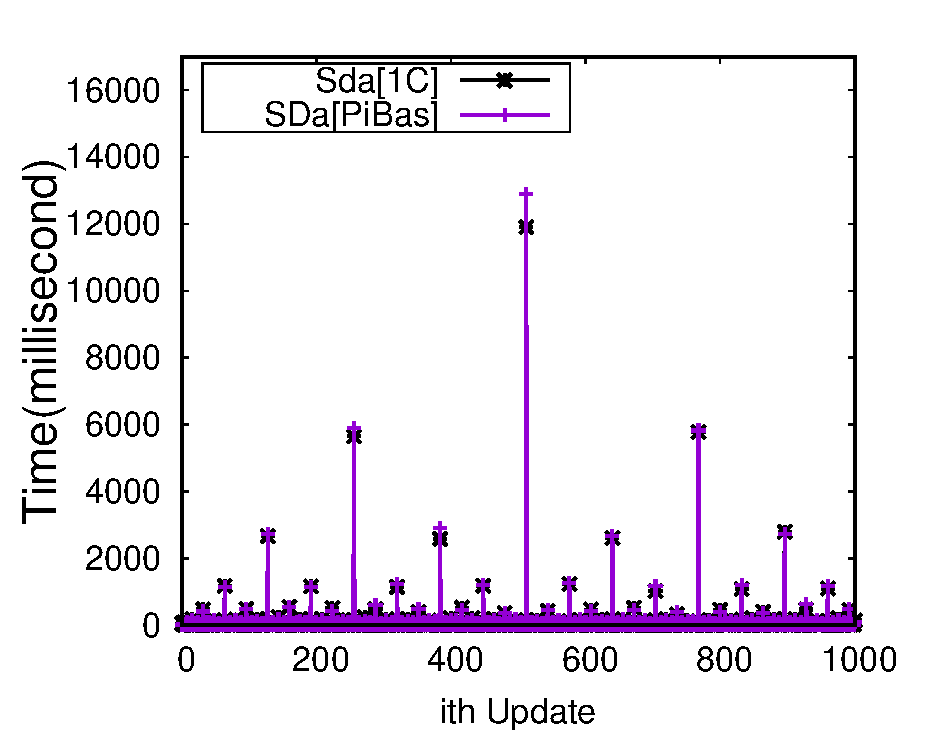
\includegraphics[width=\textwidth]{chapters/iodse/figures/Insert-SDA2.eps}
		\vspace{-0.6cm}
		\caption{}
	\end{subfigure}
 \begin{subfigure}[t]{0.48\linewidth}
		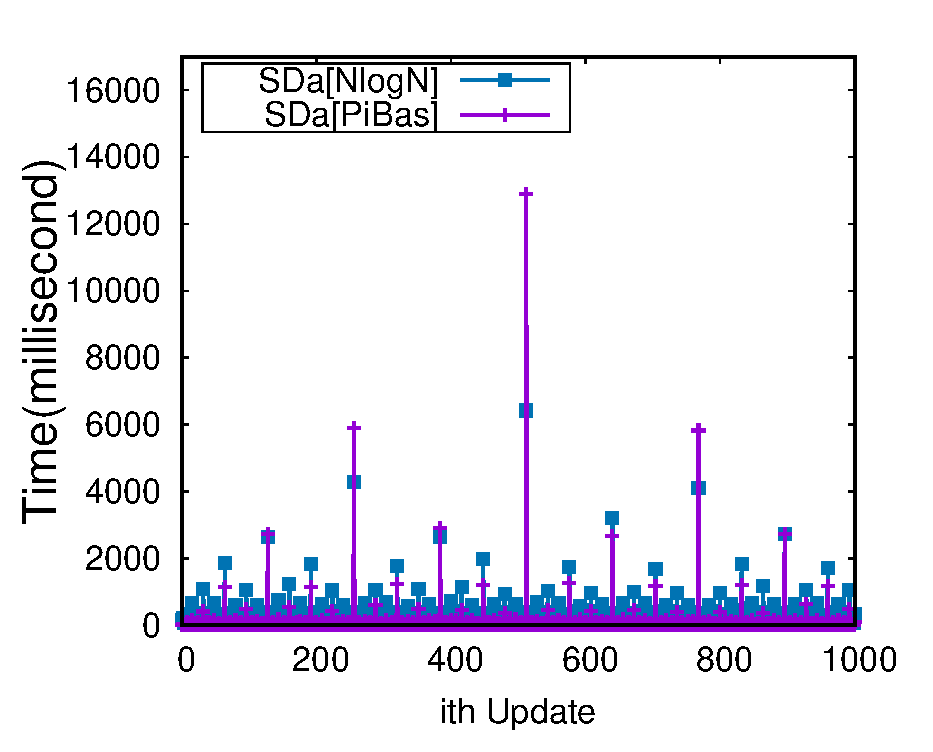
\includegraphics[width=\textwidth]{chapters/iodse/figures/Insert-SDA3.eps}
		\vspace{-0.6cm}
		\caption{}
	\end{subfigure}
	\vspace{-.3cm}
	\caption{Update computation time of amortized schemes for 1K updates starting from an empty dataset (a) \SDa[\OneChoice] vs \SDa[\PiBas] (b) \SDa[\NlogN] vs \SDa[\PiBas] }
	\label{app-fig:update}
% 	\vspace{-.3cm}
\end{figure}

\begin{figure}[t]
	\centering
 \begin{subfigure}[t]{0.48\linewidth}
		\includegraphics[width=\textwidth]{chapters/iodse/figures/UpdateTime.eps}
		\vspace{-0.6cm}
		\caption{}
	\end{subfigure}
 \begin{subfigure}[t]{0.48\linewidth}
		\includegraphics[width=\textwidth]{chapters/iodse/figures/UpdateTime-WAN1.eps}
		\vspace{-0.6cm}
		\caption{}
	\end{subfigure}
	\vspace{-.3cm}	
	\caption{Update computation time for variable database sizes (a) over single machine (b) over WAN machines with 24.7ms network delay and 2.5Gbps bandwidth.}
	\label{fig:wan}
% 	\vspace{-.3cm}
\end{figure}

% \parhead{Amortize Update Cost} Figure~\ref{fig:update}(a) shows \SDa[\NlogN] and \SDa[\PiBas] update time for 1K consecutive updates. In each update, the client fetches and merges some of the previously built levels and then uploads them to the server. Clearly, the update cost depends on the number of previously inserted indexes and increases when more number of indexes need to be merged. We repeated the same experiment for \SDa[\OneChoice] and \SDa[\TwoChoice]. However, since these two schemes show similar behavior to \SDa[\NlogN] and \SDa[\PiBas], we only provide the numbers of the aforementioned scheme which have the minimum and maximum of the update time. As is clear from the figure, as expected, \SDa[\PiBas] has the best update cost for small merges (due to the smallest number of needed entries) and the worst update cost for big merges (due to the random disk accesses). In this experiment, the minimum and maximum observed update time are $2$ms and $15143$ms.

% \begin{figure}
% \centering
% 		\includegraphics[width=0.5\linewidth]{figures/UpdateTime.eps}
% 		%\vspace{-.6cm}
% 		\caption{Update computation time for the de-amortized schemes}
%   \label{fig:updatedeam}
% \end{figure}%

% \begin{figure}[ht]
% 	\centering
% 	\begin{subfigure}[t]{0.48\linewidth}
% 		\includegraphics[width=\textwidth]{figures/UpdateTime.eps}
% 		\vspace{-0.6cm}
% 		\caption{}
% 	\end{subfigure}
%  \begin{subfigure}[t]{0.48\linewidth}
% 		\includegraphics[width=\textwidth]{figures/UpdateTime-WAN1.eps}
% 		\vspace{-0.6cm}
% 		\caption{}
% 	\end{subfigure}
% 	\vspace{-.3cm}
% 	\caption{Update computation time for the de-amortized schemes (a) on a single machine (b) on separate client/server machines with 24.7ms network delay and 2.5Gbps bandwidth.}
% 	\label{fig:updatedeam}
% % 	\vspace{-.3cm}
% \end{figure}
	

\smallskip\noindent\textbf{Update Cost of De-Amortized schemes.} To measure the update performance of our de-amortized schemes, first we measured the update computation time for variable database sizes in memory. According to our experiment (Figure~\ref{fig:wan} (a)), \LSDd[\OneChoice] outperforms other schemes for database sizes above $100K$ which is compatible with its better asymptotics (e.g., \LSDd[\OneChoice] is up to {$2.5\times$} faster than \SDd[\PiBas]\ for database size of 5M). Furthermore, \LSDd[\NlogN] has the worst performance in the memory setting due to the large number of layers it needs to create for each level of the de-amortized framework. \neww{We also provided \LSDd[\PiBas] update time to show our framework is applicable to \SDd[\PiBas] and can reduce its cost from $O(\log^3 N)$ to $O(\log^2 N)$.}
Finally, we re-executed this using HDD storage. We observe that \LSDd[\OneChoice] is still the most efficient scheme in all database sizes. On the other hand, \LSDd[\NlogN] becomes better than \SDd[\PiBas] in bigger database sizes due to its better locality (e.g., \LSDd[\OneChoice] and \LSDd[\NlogN] are {$123\times$ and $5\times$} faster than \SDd[\PiBas]\ for size 5M).


\smallskip\noindent\textbf{Update Over WAN.}
\neww{We measured end-to-end update times when client and server are located on different AWS machines, as above (Figure~\ref{fig:wan} (b)). The performance of memory-based \SDd[\PiBas] worsens due to the round trips for OMAP access and the amount of data that must be transferred over the network (\LSDd[\OneChoice] is {$8-11.3\times$} and \LSDd[\NlogN] is {$1.2-2\times$} faster than \SDd[\PiBas]). That said, the performance of disk-based schemes is similar to the single-machine case as the disk overhead is the dominant cost and the bandwidth is high enough to ``cover'' for the network overhead.}

% \begin{figure*}[ht]
% 	\centering
% 	\begin{subfigure}[t]{0.24\linewidth}
% 		\includegraphics[width=\textwidth]{figures/Search-Comp-DBSize10M-ResultSizeVar-32B-NoCache.eps}
% 		\vspace{-0.8cm}
% 		\caption{}
% 	\end{subfigure}
% 	\begin{subfigure}[t]{0.24\linewidth}
% 		\includegraphics[width=\textwidth]{figures/Search-10pCache.eps}
% 		\vspace{-.8cm}
% 		\caption{}
% 	\end{subfigure}%
% 		\begin{subfigure}[t]{0.24\linewidth}
% 		\includegraphics[width=\textwidth]{figures/Search-20pCache.eps}
% 		\vspace{-.8cm}
% 		\caption{}
% 	\end{subfigure}~
%  	\begin{subfigure}[t]{0.24\linewidth}
% 		\includegraphics[width=\textwidth]{figures/Search-50pCache.eps}
% 		\vspace{-.8cm}
% 		\caption{}
% 	\end{subfigure}~\\
% 	\vspace{-.4cm}
% 	\caption{Search computation time for $|{DB}|=2^{23}$ and variable result size for $|block|=32$B in HDD, (a) 0\% Caching, (b) 10\% Caching, (c) 20\% Caching, (c) 50\% Caching.}
% 	\label{fig:search-var-block}
% 	\vspace{-.2cm}
% \end{figure*}
% we simulated the worst-case number of IO operations they need for each update and compared them in Figure~\ref{fig:update}(b). In this Figure, we provide two simulations. First we assume that the main memory can keep constant number of entries (e.g., $M=2$ entries). In this case, all operations in all schemes would need an IO access because they cannot be kept in the main memory. Therefore, as the figure shows, \SDd[\OneChoice] will be more affected than \SDd[\PiBas] by this  because it needs to do some extra operations like sorting to provide better locality. On the other hand, \SDd[\OneChoice]s would need less number of IO operations than \SDd[\PiBas] and \SDd[\OneChoice] because it does not need OMAP and most of the update cost comes from the OMAP accesses ($\bO(\log^2N)$).

% In the second simulation, we assume that the main memory can keep $\bO(\gamma)$ number of entries. Note that this assumption mostly helps our schemes because the cost of \SDd[\PiBas] does not depends on the available main memory (even in the OMAP part it does not improve the performance). As the figure shows, this amount of memory improve the performance of \SDd[\OneChoice]s because it can execute the sort algorithm more efficiently and does not need to swap-in/out into the hard disk. Therefore, this assumption leads to more than three orders of magnitude less IO in comparison to \SDd[\PiBas]. E.g., in a dataset with size $10^7$, \SDd[\PiBas] needs 150K IOs while \SDd[\OneChoice]s only needs 144 IOs.




\vspace{-10pt}
\section{Conclusion }\vspace{-10pt}
\new{
% While forward-privacy and I/O-efficiency have been described as two 
% \emph{irreconcilable} notions in prior literature,  I
In this work,  
we proposed the first I/O efficient DSE schemes with forward/backward privacy  
by re-visiting prior ``static-to-dynamic" compilers.
% compilers presented by Demertzis et al. \cite{SDa},
% namely the \SDa\ and \SDd\ schemes. 
% These schemes originally were instantiated 
% only with \PiBas, a static SE scheme that offers worst-case I/O efficiency.  
% We observed that \SDa\ can be instantiated with any I/O-efficient static SE scheme to achieve an 
% I/O-efficient DSE scheme that also ensures forward/backward privacy. 
% The only drawback of \SDa\ is that it offers amortized update cost. 
% To overcome this problem, the natural approach was to use the \SDd\ scheme, 
% that de-amortizes the update cost, although we had to incorporate new techniques 
% to it to get it work with the I/O-efficient schemes efficiently. 
First, we came up with a new \emph{oblivious merge} framework, that enabled us to 
place entries for the same keyword close to each other (preserving locality).
Moreover, we optimized performance by replacing oblivious data structures 
% utilized in the original \SDd\cite{SDa} approach. Instead, we opted 
for more lightweight and easier-to-implement oblivious sorting algorithms and linear scans. 
% We named this modified \emph{locality-aware} scheme \LSDd\ as it is influenced from \SDd. 
We implemented both amortized and de-amortized 
% \SDa[$\cdot$] and \LSDd[$\cdot$]\ 
transformations with I/O-efficient static
schemes, such as \OneChoice, \TwoChoice, \NlogN, and \sN~(for s = 3 and 6), and compared 
their search and update times with prior works, overall showcasing our schemes' superior performance in various settings and configurations.
% the original \PiBas\ specific 
% \SDa\ and \SDd\ of \cite{SDa}. 
% Our experiments were performed for variable result size, variable database size and variable block size. 
% We conclude that the I/O-efficient schemes always 
% performed better than the non I/O-efficient ones (both for HDDs and SSDs).
}


%\tgreen{conclusion is vague}
%In this paper, we proposed two families of I/O efficient DSE schemes with 
%forward/backward privacy. The first proposes a static-to-dynamic transformation with amortized update %cost. The second is aiming for schemes with de-amortized update costs proposing a new strategy based on %oblivious sorting. We show that our proposed constructions improve state-of-the art both experimentally %and asymptotically. 

